\documentclass[conference]{IEEEtran}
\IEEEoverridecommandlockouts
\usepackage[T1]{fontenc}
\usepackage{cite}
\usepackage{amsmath,amssymb,amsfonts}
\usepackage{graphicx}
\usepackage{textcomp}
\usepackage{xcolor}
\usepackage{booktabs}
\usepackage{multirow}
\usepackage{array}
\usepackage{microtype}

\emergencystretch=1.5em

\def\BibTeX{{\rm B\kern-.05em{\sc i\kern-.025em b}\kern-.08em
    T\kern-.1667em\lower.7ex\hbox{E}\kern-.125emX}}

\newcommand{\pmtwofive}{PM$_{2.5}$}

\begin{document}

\title{
  Auditing Spatial Shortcuts, Prototype Multitask Regularization, and Multimodal
  Fusion for Global Street-Level Air Quality Estimation
}

\author{
  \IEEEauthorblockN{Mughilvannan Manivannan}
  \IEEEauthorblockA{\textit{Dept. of Computer Science} \\
    \textit{OsloMet University}\\ Oslo, Norway \\ muman2187@oslomet.no}
  \and \IEEEauthorblockN{Ahamed Hasan}
  \IEEEauthorblockA{\textit{Dept. of Computer Science} \\
    \textit{OsloMet University}\\ Oslo, Norway \\ ahhas2658@oslomet.no}
  \and \IEEEauthorblockN{Mrinmoy Das}
  \IEEEauthorblockA{\textit{Dept. of Computer Science} \\
    \textit{OsloMet University}\\ Oslo, Norway \\ mrdas1414@oslomet.no}
}

\maketitle

\begin{abstract}
  Estimating ambient fine particulate matter (\pmtwofive) and US Environmental
  Protection Agency (EPA) Air Quality Index (AQI) levels directly from daytime
  street-level photographs offers an inexpensive, high-density complement to
  sparse regulatory monitoring networks. However, evaluating computer-vision AQI
  models on global crowdsourced datasets introduces severe methodological
  pitfalls: stationary camera overlap, urban geospatial shortcuts, and
  validation-loss checkpointing artifacts can make models appear accurate even
  when they fail to learn physical atmospheric scattering cues. In this study,
  we conduct a rigorous empirical investigation on the global crowdsourced
  PM25Vision benchmark (8,176 cleaned training images across 2,527 primary
  stations and 2,920 test images across 729 stations, including an unseen-region
  subset of 717 images across 205 stations located more than 25~km from any
  training station). Building upon two recent IEEE Transactions frameworks---the
  Multiscale Dilated Network (MDNet) and the Prototype Feature
  Representation-Guided Multitask Learning (PFRML) architecture---alongside
  domain-specific attention, physics-gating, and class-weighting mechanisms, we
  evaluate five progressive experiment families under leakage-free 5-fold
  station-grouped and 25~km spatial-cluster cross-validation, strict last-epoch
  reporting, and 1,000-resample station-level cluster bootstrapping. Four key
  findings emerge. First, a non-visual 5-input GPS-and-month Multi-Layer
  Perceptron (Metadata MLP) achieves a deceptively strong 40.34 Mean Absolute
  Error (MAE) ($R^2 = 0.4982$) on the full test set by interpolating nearby
  urban stations, but collapses completely on stations more than 25~km away (MAE
  $= 49.84$, $R^2 = -0.0393$). Second, among vision-only models, ImageNet
  pretraining is the dominant performance driver, reducing 5-fold station
  cross-validation MAE by 7.61 to 9.24 AQI points (44.05--45.66 for pretrained
  ResNet-18, our MobileNetV3-S + MD-Neck adaptation, and MobileNetV3-Small
  vs.\ 53.27--53.29 for from-scratch ResNet-18 and MDNet-T). Third, across a
  controlled 5-fold ablation ladder, PFRML's multi-stage Dimension Consistency
  Module and Transformer neck without prototypes (R1, MAE $= 45.50 \pm 8.64$)
  matches the pretrained backbone, whereas enabling the 6-class prototype
  multitask head (R2, $48.14 \pm 7.61$; literal Eq.~5 variant, $48.04 \pm 8.20$)
  consistently degrades continuous AQI regression by 2.54 to 2.63 MAE points,
  and plain pretrained MobileNetV3-Small significantly outperforms the full
  PFRML model on the held-out test set (MAE $= 41.12$ vs.\ $45.04$, paired 95\%
  confidence interval $[-6.27, -1.58]$) and beyond 25~km ($39.60$ vs.\ $46.79$,
  $[-11.92, -2.53]$). Fourth, fusing the prototype-free R1 visual spine with
  metadata under an early-stopped 7-epoch schedule selected via centered moving
  average achieves the lowest overall test MAE ($35.77\;[30.47, 42.72]$,
  $R^2 = 0.6070$), significantly beating both single modalities on the full test
  set ($-4.57\;[-8.31, -1.26]$ vs.\ metadata-only; $-5.35\;[-8.62, -2.26]$
  vs.\ image-only) and tying the plain image model at $> 25$~km ($39.22$
  vs.\ $39.60$), though metadata-zeroed evaluation ($47.56$ test MAE) reveals
  that the fused regression head still relies heavily on geospatial coordinates.
\end{abstract}

\begin{IEEEkeywords}
  Air Quality Index (AQI), \pmtwofive{} estimation, multiscale dilated
  convolution, prototype multitask learning, multimodal fusion, spatial
  generalization, shortcut learning.
\end{IEEEkeywords}

\section{Introduction}
\label{sec:introduction}

Fine particulate matter with an aerodynamic diameter of 2.5~$\mu$m or less
(\pmtwofive) is a primary environmental risk factor for cardiovascular and
respiratory morbidity worldwide. Reference-grade gravimetric and
beta-attenuation monitoring stations provide accurate hourly measurements, yet
high installation and maintenance costs severely restrict their spatial
coverage. Even in densely populated metropolitan basins, monitoring stations are
often separated by several kilometers, while vast peri-urban and rural regions
remain completely unmonitored. Consequently, estimating outdoor air pollution
directly from ground-level daytime photographs captured by smartphones, traffic
cameras, or crowdsourced mapping platforms has emerged as a promising paradigm
for scalable environmental sensing~\cite{marzaguiReviewImageQuality2024,
wangLightweightAirQuality2024, wangPrototypeFeatureRepresentationGuided2026}.

The physical foundation for visual air quality estimation lies in atmospheric
optics. Airborne \pmtwofive{} aerosols have radii comparable to the wavelength
of visible light (0.4--0.7~$\mu$m) and therefore attenuate and scatter sunlight
primarily via Mie scattering, governed macroscopically by the Beer--Lambert law
and Koschmieder's atmospheric visibility
model~\cite{marzaguiReviewImageQuality2024, yadavRoadsideTreeImageBased2025}. As
particulate concentration increases, airlight scattered along the line of sight
brightens dark shadow regions (the basis of the Dark Channel Prior), washes out
color saturation in the sky and distant vegetation, and degrades high-frequency
edge contrast along building skylines and
horizons~\cite{chakrabortyCanImageTell2024, dohaDeepMultiTaskLearning2026}. In
machine learning terms, inferring a continuous pollution score such as the US
Environmental Protection Agency (EPA) Air Quality Index (AQI, ranging from 0 to
over 500) is formulated as a regression task, whereas assigning a scene to one
of the six official US EPA health advisory categories---\textit{Good} (0--50),
\textit{Moderate} (51--100), \textit{Unhealthy for Sensitive Groups (USG)}
(101--150), \textit{Unhealthy} (151--200), \textit{Very Unhealthy} (201--300),
and \textit{Hazardous} ($> 300$)---is formulated as a 6-class classification
task~\cite{wangLightweightAirQuality2024,
wangPrototypeFeatureRepresentationGuided2026}.

Despite rapid progress from handcrafted optical
descriptors~\cite{marzaguiReviewImageQuality2024, chakrabortyCanImageTell2024,
yadavRoadsideTreeImageBased2025} to deep convolutional neural networks
(CNNs)~\cite{kaushalEvaluationDeepLearning2024, vermaImagebasedAirPollution2025,
kumaar.bImageBasedAir2025, zhangAirQualityLevel2024}, physics-guided
hybrids~\cite{dohaDeepMultiTaskLearning2026, razimiIntegratingDeepLearning2024a,
leeEnhancingPM25Detection2025}, and multimodal or contrastive
frameworks~\cite{abdelsalamSkyFuseNetCrossAttentionSwin2026,
kambleMobileImageDrivenPM252025, hanSmartCamAirDetectContrastiveApproach2025,
mohanDeepLearningBasedPM252025, vahdatpourForecastingVisualizingAir2025},
deploying image-based AQI models in the wild faces a fundamental validity
crisis. Most published studies train and evaluate on fixed cameras from a single
city or a handful of stationary sites. When evaluated under random image-level
splits, high-capacity networks easily memorize static background landmarks
(buildings, trees, road geometry) and camera color profiles rather than
atmospheric haze. When recent studies enforced strict location-disjoint
evaluation---such as Nathvani et al.~\cite{nathvaniHereNowEvaluating2023} across
1.6 million street-view images in Accra, Ghana, or Byler et
al.~\cite{bylerLocationGeneralizabilityImageBased2025} across 15 US National
Parks---classification accuracy dropped sharply on unseen sites.

Transitioning from local fixed-camera datasets to a global crowdsourced
street-level dataset such as PM25Vision introduces two major scientific
challenges that motivate our work:
\begin{enumerate}
  \item \textbf{Visual heterogeneity and domain noise:} Crowdsourced street
        photographs span thousands of distinct cameras, exposure settings,
        viewing angles, urban architectures, and weather patterns. An overcast
        sky in a clean maritime climate can appear visually greyer than a sunny
        winter day in a polluted continental basin, confounding simple haze
        heuristics.
  \item \textbf{The geospatial and seasonal shortcut:} In machine learning, a
        \textit{shortcut} (or spurious correlation) occurs when an easily
        memorized non-causal attribute allows a network to minimize training
        loss without learning the underlying physical task. Because air
        pollution is strongly regional and seasonal, and because crowdsourced
        test stations frequently sit within the same cities as training
        stations, a model supplied with sample metadata (such as GPS coordinates
        and capture month) can achieve low error simply by memorizing
        \textit{where} and \textit{when} a photograph was taken, without
        extracting any visual haze information from the pixels.
\end{enumerate}

To investigate these challenges systematically, we center our architectural
study on two core IEEE Transactions papers examined in detail in our companion
Literature Review: (1) the \textbf{Multiscale Dilated Network (MDNet)} by Wang
et al.~\cite{wangLightweightAirQuality2024} (\textit{IEEE Trans.\ Ind.\ Inf.},
2024), which uses parallel depthwise dilated convolutional blocks (MDBlock) to
expand the receptive field for global sky-to-ground haze extraction with minimal
parameters; and (2) the \textbf{Prototype Feature Representation-Guided
Multitask Learning (PFRML)} framework by Wang et
al.~\cite{wangPrototypeFeatureRepresentationGuided2026} (\textit{IEEE
Trans.\ Geosci.\ Remote Sens.}, 2026), which fuses four hierarchical backbone
stages through a Dimension Consistency Module (DCM) and a Transformer encoder,
and regularizes continuous regression via a 6-class Exponential Moving Average
(EMA) prototype classification head under a hybrid multitask loss. Onto this
two-paper spine, we integrate and ablate three domain-specific mechanisms from
the broader literature: learnable spatial token attention
pooling~\cite{abdelsalamSkyFuseNetCrossAttentionSwin2026,
leeEnhancingPM25Detection2025}, differentiable atmospheric physics
gating~\cite{dohaDeepMultiTaskLearning2026, yadavRoadsideTreeImageBased2025,
marzaguiReviewImageQuality2024}, and fold-internal inverse-frequency class
weighting~\cite{dohaDeepMultiTaskLearning2026,
bylerLocationGeneralizabilityImageBased2025, mohanDeepLearningBasedPM252025}.

Rather than assuming that complex architectural modules automatically transfer
to global crowdsourced imagery, we design a strictly controlled empirical
protocol around four research questions:
\begin{itemize}
  \item \textbf{RQ1 (The Geospatial Shortcut vs.\ Visual Generalization):} How
        much predictive skill on PM25Vision can be achieved by non-visual GPS
        and seasonal metadata alone compared to handcrafted optical statistics
        and deep vision models, and what happens to each modality when evaluated
        on unseen regions more than 25~km from any training station?
  \item \textbf{RQ2 (Transfer Learning vs.\ From-Scratch Domain CNNs):} On
        roughly 8,200 heterogeneous street scenes, how does Paper~2's
        from-scratch multiscale dilated backbone (MDNet-T) compare against
        ImageNet-pretrained backbones (ResNet-18, MobileNetV3-Small) and our own
        hybrid adaptation (MobileNetV3-S + MD-Neck) that grafts multiscale
        dilated blocks onto pretrained features?
  \item \textbf{RQ3 (Prototype Multitask Regularization and Literature
        Toggles):} Across a 5-fold station-disjoint ablation ladder, do PFRML's
        multi-stage DCM + Transformer neck (R1), its 6-class EMA prototype
        multitask head (R2, in both prototype-weighted and literal Eq.~5 forms),
        and literature toggles (attention pooling, physics prior gate, class
        weights, DCM concatenation) improve continuous AQI regression over a
        plain pretrained backbone?
  \item \textbf{RQ4 (Multimodal Fusion and Shortcut Reliance):} Can combining
        visual features with GPS/month metadata under 25~km spatial-cluster
        cross-validation, modality dropout, a detached auxiliary vision loss,
        and early stopping outperform both single modalities on held-out test
        stations without collapsing in unseen regions---and how much does the
        resulting fusion model still rely on location when metadata is zeroed at
        test time?
\end{itemize}

The remainder of this report is organized as follows.
Section~\ref{sec:data_methodology} details the PM25Vision dataset audit,
deterministic cleaning, physics-preserving preprocessing, dual group-split
cross-validation and statistical protocols, and the architecture of all
baseline, backbone, PFRML, and multimodal fusion models.
Section~\ref{sec:results} presents the quantitative results across all five
experiment groups, failure diagnostics, and an evidence-based discussion of
limitations and threats to validity. Section~\ref{sec:conclusion} summarizes our
conclusions and reproducibility specifications.

\section{Data and Methodology}
\label{sec:data_methodology}

\subsection{Dataset Audit and Deterministic Cleaning (PM25Vision)}
\label{subsec:dataset_cleaning}

We conduct all experiments on the global crowdsourced PM25Vision dataset
(sourced from Hugging Face Hub, DeadCardassian/PM25Vision). The dataset pairs
daytime street-level RGB photographs with ground-truth pollution measurements
and metadata including station identifier, geographic coordinates (latitude and
longitude), and capture timestamp. Although the target column in the raw CSV
files is labeled \texttt{pm25}, its continuous values span 1.0 to 530.0 and
follow the official threshold boundaries of the \textbf{US EPA Air Quality Index
(AQI)} scale across six ordinal health categories (Bins 1--6, indexed 0 to 5):
\textit{Good} (0--50), \textit{Moderate} (51--100), \textit{Unhealthy for
Sensitive Groups} (101--150), \textit{Unhealthy} (151--200), \textit{Very
Unhealthy} (201--300), and \textit{Hazardous}
(301--600)~\cite{wangLightweightAirQuality2024,
wangPrototypeFeatureRepresentationGuided2026}.

A forensic audit of the raw metadata files (8,298 training rows across 8,194
unique image IDs and 2,532 raw stations; 2,921 test rows across 2,920 unique
image IDs and 729 stations; 3,261 raw unique stations total) uncovered two
sources of data leakage and label ambiguity:
\begin{enumerate}
  \item \textbf{Cross-split image leakage:} Exactly 18 unique image IDs appeared
        in both the training and test splits. Leaving identical photographs in
        both splits would directly leak test images into training.
  \item \textbf{Multi-station duplicate rows:} Within both splits, several image
        IDs were duplicated across multiple rows matched to different nearby
        monitoring stations with slightly different AQI readings.
\end{enumerate}

To guarantee a leakage-free benchmark, our deterministic cleaning pipeline
executes two operations before any splitting or model training:
\begin{enumerate}
  \item \textbf{Overlap purging:} All rows corresponding to the 18 cross-split
        overlapping image IDs are removed strictly from the training split,
        leaving 3,259 unique audited stations (2,530 in train and 729 in test)
        with zero shared images or stations between train and test.
  \item \textbf{Median-AQI deduplication:} Within each split independently, rows
        are sorted deterministically by image ID and station ID. For any image
        appearing multiple times, its continuous AQI label is replaced by the
        \textit{median} AQI across its duplicate rows (preventing extreme sensor
        outliers from skewing the target), the first sorted station record is
        retained as the primary station ID, and the discrete 6-class AQI bin is
        recomputed from the deduplicated median AQI.
\end{enumerate}

After deterministic cleaning, the dataset comprises \textbf{11,096 unique
images} partitioned into:
\begin{itemize}
  \item \textbf{Cleaned Training Set:} $n = 8,176$ unique images across 2,527
        primary stations (mean AQI $= 121.80 \pm 88.35$, median $= 111.00$).
  \item \textbf{Cleaned Test Set (\texttt{test}):} $n = 2,920$ unique images
        across 729 stations (zero overlap with training images or stations).
  \item \textbf{Unseen-Region Test Subset (\texttt{test\_gt25km}):} To evaluate
        true regional generalization where city-level coordinate interpolation
        fails, we compute the exact great-circle Haversine distance from every
        test image to its nearest cleaned training image and isolate all test
        samples located strictly more than 25.0~km from the closest training
        sample, yielding $n = 717$ images across 205 stations.
\end{itemize}

Across the 8,176 cleaned training images, the first four US EPA bins (AQI
$\le 200$) are nearly uniformly distributed: Bin~1 (\textit{Good}, $n = 1,778$,
21.75\%), Bin~2 (\textit{Moderate}, $n = 1,775$, 21.71\%), Bin~3 (\textit{USG},
$n = 1,760$, 21.53\%), and Bin~4 (\textit{Unhealthy}, $n = 1,777$, 21.73\%). By
contrast, severe pollution episodes form a pronounced long tail: Bin~5
(\textit{Very Unhealthy}, 201--300, $n = 731$, 8.94\%) and Bin~6
(\textit{Hazardous}, 301--600, $n = 355$, 4.34\%) together account for
\textbf{1,086 images (13.28\%)} of the training set. During neural network
training, continuous AQI targets are divided by a constant scale factor of 100.0
so that Mean Squared Error (MSE) regression loss has a magnitude comparable to
6-class cross-entropy loss; all model predictions are multiplied back by 100.0
and clipped at zero before computing evaluation metrics in native AQI units.
Fig.~\ref{fig:dataset_splits} illustrates the dataset class distribution and
nearest-station spatial separation across all splits.

\begin{figure}[t]
  \centering
  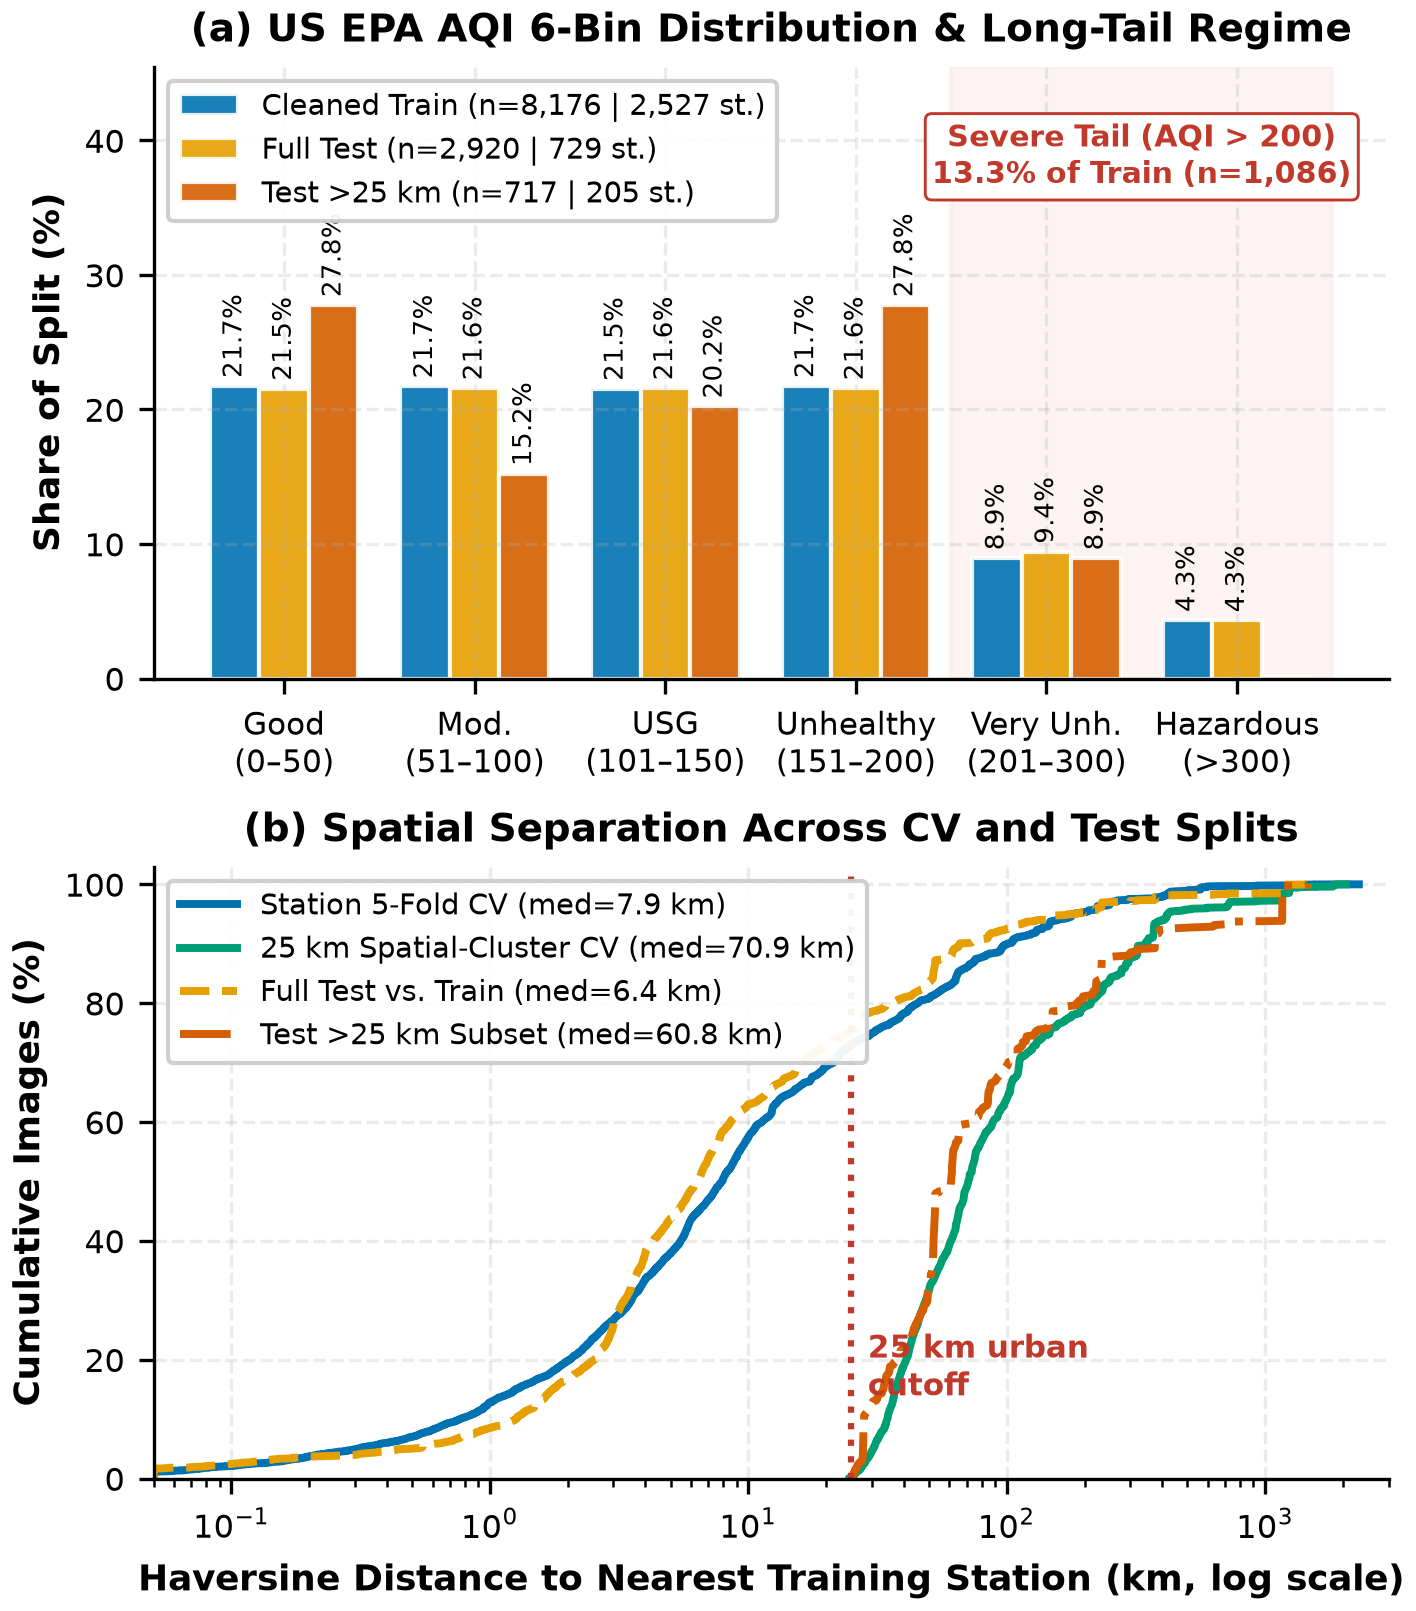
\includegraphics[width=\columnwidth]{figures/ieee_fig1_dataset_splits.png}
  \caption{
    US EPA AQI class distribution and nearest-training-station spatial
    separation across cross-validation and test partitions on cleaned
    PM25Vision.
  }
  \label{fig:dataset_splits}
\end{figure}

\subsection{
  Physics-Preserving Preprocessing and Dual Group-Split Validation Protocol
}
\label{subsec:preprocessing_splits}

\subsubsection{Physics-Preserving Image Transforms}

Standard computer-vision classification pipelines routinely apply random
cropping, color jitter (random brightness, contrast, saturation, and hue
shifts), and random grayscale conversion to force invariance to lighting and
camera differences. However, as established by Wang et
al.~\cite{wangLightweightAirQuality2024} (Sec.~III-C) and Byler et
al.~\cite{bylerLocationGeneralizabilityImageBased2025}, color saturation,
luminance contrast, and sky-to-ground brightness gradients \textit{are} the
physical Mie scattering signal encoding particulate concentration. Applying
random color jitter scrambles the optical relationship between pixel intensities
and ground-truth AQI, while random cropping frequently discards either the upper
sky region or the lower building/ground reference region.

Consequently, our transform pipeline resizes every whole photograph directly to
$224 \times 224$ pixels using antialiased bilinear interpolation without
cropping, preserving both sky and ground context. Color jitter and grayscale
conversion are strictly banned. During training, we apply only
geometry-preserving augmentations: random horizontal flipping (50\% probability)
and mild random affine perturbation (rotation within $\pm 5^\circ$, translation
within $\pm 2\%$, and scaling within 0.98--1.02), followed by standard ImageNet
channel normalization. Evaluation uses deterministic $224 \times 224$ bilinear
resize and ImageNet normalization only.

\subsubsection{Dual 5-Fold Stratified Group Cross-Validation}

Because multiple photographs originate from the same monitoring station or urban
neighborhood, random image-level splitting is prohibited throughout our study.
Instead, we partition the 8,176 cleaned training images using 5-fold Stratified
Group $K$-Fold cross-validation (stratified by the 6-class AQI bin) under two
distinct grouping modes:
\begin{enumerate}
  \item \textbf{Station-Grouped CV (\texttt{station} mode, 2,527 groups):}
        Groups samples by station ID, guaranteeing that all images from a given
        monitoring station reside in the same fold (zero station overlap between
        training and validation folds). This protocol prevents same-camera
        background memorization and is used to evaluate all vision-only
        backbones (E2, E3, E3b) and the 5-fold PFRML ablation ladder (E4).
  \item \textbf{25 km Spatial-Cluster CV (\texttt{spatial\_cluster} mode, 1,059
        groups):} Even when station IDs are disjoint, large metropolitan areas
        contain many distinct stations separated by only a few kilometers. A
        multimodal model receiving GPS coordinates can easily interpolate AQI
        from a neighboring station 2~km away under station-grouped CV. To close
        this loophole, we compute the median latitude and longitude for each
        unique station, calculate pairwise great-circle Haversine distances in
        kilometers, and group stations via single-linkage agglomerative
        clustering at a 25.0~km distance threshold. Single-linkage clustering
        merges any pair of stations within 25.0~km into the same connected urban
        cluster (1,059 clusters total across the 2,527 training stations),
        forcing entire metropolitan clusters into the same fold and testing
        whether multimodal fusion generalizes to unseen cities.
\end{enumerate}

\subsubsection{Fold-3 High-Pollution Tail Concentration Diagnostic}

An important property of group-split environmental data emerged from our fold
diagnostic audit: while Stratified Group $K$-Fold balances total validation
images (1,624--1,654 per fold), validation stations (502--508 per fold), and
head-bin counts across all five station folds, individual stations with hundreds
of severe pollution images must remain undivided inside a single fold. In Fold~3
($n = 1,646$, 503 stations, 229 Bins 5--6 images), validation AQI standard
deviation reaches 108.20 (mean 130.71) compared to 79.34--88.38 across Folds 0,
1, 2, and 4. Specifically, just four $1^\circ \times 1^\circ$ geographic grid
cells (7 stations total) concentrate \textbf{76.86\% (176 / 229)} of Fold~3's
entire Bins 5--6 tail: Delhi/NCR ($28^\circ$N, $77^\circ$E; 85 images, mean AQI
288.84, 79 tail images $= 34.50\%$), Saltillo/Monterrey ($25^\circ$N,
$-101^\circ$E; 51 images, mean AQI 474.00, 47 Bin-6 Hazardous images
$= 20.52\%$), Chiang Rai ($19^\circ$N, $99^\circ$E; 32 images, mean AQI 225.72,
31 tail images $= 13.54\%$), and Pune ($18^\circ$N, $73^\circ$E; 39 images, mean
AQI 190.18, 19 tail images $= 8.30\%$). Because even the trivial constant-median
baseline jumps from 62.31--67.18 MAE on Folds 0, 1, 2, and 4 to \textbf{74.33
MAE} on Fold~3, single-fold ablations on Fold~0 (the easiest fold for neural
models) cannot resolve 1--2 MAE differences. Every ablation rung in our study is
therefore executed across all 5 folds.

\subsubsection{Evaluation Metrics, Last-Epoch Policy, and Statistical Testing}

Every model is evaluated on a unified suite of 10 metrics computed on unscaled
native AQI values:
\begin{itemize}
  \item \textbf{Continuous regression metrics (5):} Mean Absolute Error (MAE),
        Root Mean Squared Error (RMSE), Pearson Linear Correlation Coefficient
        (PLCC), Spearman Rank Correlation Coefficient (SRCC), and Coefficient of
        Determination ($R^2$). To normalize for intrinsic fold difficulty, we
        also report the \textbf{Skill Score} relative to the constant median
        baseline:
        \begin{equation}
          \text{Skill}
          = 1 - \frac{\text{MAE}}{\text{MAE}_{\text{median}}}, \label{eq:skill}
        \end{equation}
        where $\text{Skill} = 0$ matches median guessing and $+0.33$ indicates a
        33\% error reduction.
  \item \textbf{6-class severity classification metrics (3):} Exact 6-class
        accuracy (Acc), adjacent-category accuracy within at most 1 bin
        ($\pm 1$Acc~\cite{nathvaniHereNowEvaluating2023}), and unweighted
        6-class Macro-F1. For regression-only models, predicted continuous AQI
        is mapped to the 6 discrete bins via the official US EPA thresholds; for
        multitask PFRML models, the predicted class is the prototype with
        highest softmax probability.
  \item \textbf{High-pollution tail metrics (AQI $> 200$, Bins 5--6) (2):}
        TailMAE (MAE restricted to true Bins 5--6 samples) and TailF1
        (macro-averaged $F_1$ across Bins 5 and 6).
\end{itemize}

Crucially, \textbf{all cross-validation and final test tables follow a strict
last-epoch reporting policy}. In early exploratory logs, checkpoints were saved
at the epoch minimizing validation loss. As our failure diagnostic revealed, in
multitask PFRML runs the total validation loss (classification cross-entropy
plus $0.5 \times \text{MSE}$) reaches a premature minimum at epochs 2--6
(1.53--2.13) and then rises to 2.21--2.81 by epoch 30 as the 6-class classifier
becomes overconfident on unseen stations, even while continuous validation MAE
continues improving. Moreover, on noisy Fold~3 of pretrained ResNet-18, minimum
validation loss selected epoch~1, distorting its 5-fold mean (46.16 best-epoch
vs.\ 44.05 last-epoch MAE). Finally, when training a final model once on 100\%
of the 8,176 training images for one-shot test evaluation, no validation split
exists to select a best epoch. Quoting the final epoch of the fixed cosine
learning-rate schedule eliminates checkpoint-selection bias across all
comparisons.

For statistical comparisons across $n = 5$ cross-validation folds, a two-sided
paired Wilcoxon signed-rank test has a minimum attainable $p$-value of
$2 / 2^5 = 0.0625 > 0.05$ even when one model wins all 5/5 folds. We therefore
report the \textbf{paired mean difference $\pm$ standard error
($\text{SE} = \text{SD} / \sqrt{5}$)} alongside \textbf{folds won out of 5}. For
final one-shot test evaluation, errors on multiple photographs from the same
monitoring station are correlated; resampling individual images would treat
2,920 correlated photos as independent and yield artificially narrow confidence
intervals. Instead, we compute 95\% confidence intervals (CIs) for both absolute
MAE and pairwise model differences via a \textbf{1,000-resample station-level
cluster bootstrap} ($\text{seed} = 42$), drawing 729 stations (or 205 stations
in \texttt{test\_gt25km}) with replacement on each replicate and weighting each
drawn station by all of its constituent images.

\subsection{Non-Visual Baselines and Vision-Only Backbones (E0--E3b)}
\label{subsec:baselines_backbones}

\subsubsection{Non-Visual and Handcrafted Optical Baselines (E0, E1)}

To anchor our experimental ladder, we first implement three non-deep or
non-visual baselines:
\begin{itemize}
  \item \textbf{Constant Median Predictor (\texttt{E0\_median}):} Outputs the
        constant median AQI of the active training split (110.00--112.00 across
        CV folds), establishing the zero-skill error floor.
  \item \textbf{Haze-Statistics Ridge Regression (\texttt{E0\_ridge}):} A
        deterministic PyTorch feature extractor computes three pixel-level
        physical haze maps on pre-normalization RGB images in $[0, 1]$: HSV
        color saturation, Sobel luminance edge-gradient contrast, and the
        $15 \times 15$ patch-wise Dark Channel
        Prior~\cite{marzaguiReviewImageQuality2024,
        wangPrototypeFeatureRepresentationGuided2026}. To capture
        sky-versus-ground differentials~\cite{chakrabortyCanImageTell2024,
        vahdatpourForecastingVisualizingAir2025}, the mean and standard
        deviation of each map are pooled over three horizontal image bands (full
        image, top sky half, and bottom ground half), yielding
        $3 \times 3 \times 2 = 18$ interpretable optical features. A
        standardized Ridge regression pipeline (\texttt{RidgeCV}) selects the
        $L_2$ regularization penalty
        $\alpha \in \{0.01, 0.1, 1, 10, 100, 1000\}$ strictly within each
        training fold.
  \item \textbf{GPS + Month Metadata MLP (\texttt{E1\_metadata\_mlp}):} To
        quantify the pure geospatial and seasonal shortcut without looking at a
        single pixel, we encode station latitude and longitude as 3D unit-sphere
        Cartesian coordinates $(x, y, z)$ (avoiding the $\pm 180^\circ$
        longitude discontinuity) and capture month $m \in \{1,\dots,12\}$ as a
        cyclic sine/cosine pair $(\sin(2\pi m/12), \cos(2\pi m/12))$. This
        5-input vector passes through a two-hidden-layer ReLU MLP
        ($5 \to 64 \to 32 \to 1$; 2,497 parameters), trained for 40 epochs with
        AdamW ($\text{lr} = 10^{-3}$, weight decay $10^{-4}$, cosine annealing)
        under scaled MSE loss.
\end{itemize}

\subsubsection{
  Vision-Only Backbones and Our MobileNetV3-S + MD-Neck Adaptation (E2, E3, E3b)
}

To test RQ2 (transfer learning versus custom dilated atmospheric CNNs), we
compare five vision-only regression families trained under 5-fold
station-grouped CV:
\begin{enumerate}
  \item \textbf{Pretrained and From-Scratch Standard Backbones (E2):} We
        evaluate ResNet-18 (11.18M parameters, linear head $512 \to 1$) both
        from random initialization (\texttt{E2\_resnet18\_scratch}) and with
        ImageNet-1K pretrained weights (\texttt{E2\_resnet18\_pretrained}), as
        well as ImageNet-pretrained MobileNetV3-Small (\texttt{E2}, 1.52M
        parameters, classifier head $1024 \to 1$).
  \item \textbf{From-Scratch Multiscale Dilated Network (E3, Paper~2 MDNet-T):}
        Following Wang et al.~\cite{wangLightweightAirQuality2024}
        (Sec.~III-A/B, Table~I), we implement the 4-stage MDNet-T hierarchy
        (stage depths $[3, 3, 9, 3]$, channel widths $[96, 192, 384, 768]$,
        4.93M parameters). A $4 \times 4$ stride-4 patchify stem and three
        inter-stage $2 \times 2$ stride-2 downsampling layers produce feature
        maps at spatial resolutions $56 \times 56$, $28 \times 28$,
        $14 \times 14$, and $7 \times 7$. Within each stage, every Multiscale
        Dilated Block (MDBlock) processes its input through three parallel
        depthwise dilated convolutional branches with kernel sizes and dilation
        rates $(k = 3, d = 2)$, $(k = 2, d = 2)$, and
        $(k = 1, d = 1)$---corresponding to effective receptive windows of
        $5 \times 5$, $3 \times 3$, and $1 \times 1$---sums their outputs,
        applies GELU activation, a $1 \times 1$ pointwise convolution,
        channel-wise 2D LayerNorm, and a residual shortcut connection. Across
        its 18 blocks, MDNet-T achieves a theoretical receptive field of 1,136
        pixels. Because no ImageNet pretrained weights exist for MDNet-T, it is
        initialized randomly and trained from scratch.
  \item \textbf{Authors' Adaptation: Pretrained MobileNetV3-S + MD-Neck (E3b):}
        Training a 4.93M-parameter CNN from scratch on roughly 6,540 per-fold
        training images is severely data-limited. To test Paper~2's multiscale
        dilated block concept on top of transferred visual features, we designed
        our own adaptation (\texttt{MobileNetV3MDNeck}, experiment
        \texttt{E3b}). \textit{We explicitly state that E3b is our own
        architectural adaptation and is not a model from the original MDNet
        paper~\cite{wangLightweightAirQuality2024}.} It extracts the stride-32
        feature map ($576 \times 7 \times 7$) from an ImageNet-pretrained
        MobileNetV3-Small backbone, applies a $1 \times 1$ convolutional channel
        reduction ($576 \to 128$) and 2D LayerNorm, passes the features through
        2 sequential MDBlock(128) layers, applies Global Average Pooling (GAP)
        and LayerNorm, and predicts scaled AQI via a linear head ($128 \to 1$;
        1.04M total parameters).
\end{enumerate}

To select learning rates and epoch counts without peeking at the test set, our
baseline queue enforced a pre-committed 3-stage rule: Stage~1 screened candidate
schedules ($\text{lr} \in \{10^{-3}, 3 \times 10^{-4}\}$, epochs
$\in \{30, 40, 60\}$) on Fold~0 only; Stage~2 switched a model family away from
the default ($\text{lr} = 10^{-3}$, 30 epochs) \textit{if and only if} the
candidate lowered Fold-0 validation MAE by at least 1.0 AQI point; and Stage~3
executed full 5-fold station CV for the selected configurations.

\subsection{Unified PFRML Visual Spine and Literature Toolbox Toggles (E4, E5)}
\label{subsec:pfrml_methodology}

To evaluate RQ3, we implement a backbone-agnostic PFRML
framework~\cite{wangPrototypeFeatureRepresentationGuided2026}. Whereas the
original PFRML paper pairs a ResNet-50 backbone with a 12-layer Vision
Transformer (115.2M parameters, trained at $\text{lr} = 2 \times 10^{-4}$, batch
size 16, and a $1024 \to 256 \to 1$ regression MLP), we substitute
ImageNet-pretrained MobileNetV3-Small (stage channels $[16, 24, 48, 576]$ at
strides $[4, 8, 16, 32]$; $\sim 2.0\text{M}$ total parameters) as our primary
backbone so that all 5-fold ablations share the exact training schedule of our
pretrained MobileNetV3-Small baseline ($\text{lr} = 10^{-3}$, 30 epochs with
3-epoch linear warmup, batch size 32, \texttt{fp32}), and we also evaluate PFRML
on from-scratch MDNet-T. Fig.~\ref{fig:architecture} illustrates the complete
system architecture.

\begin{figure*}[t]
  \centering
  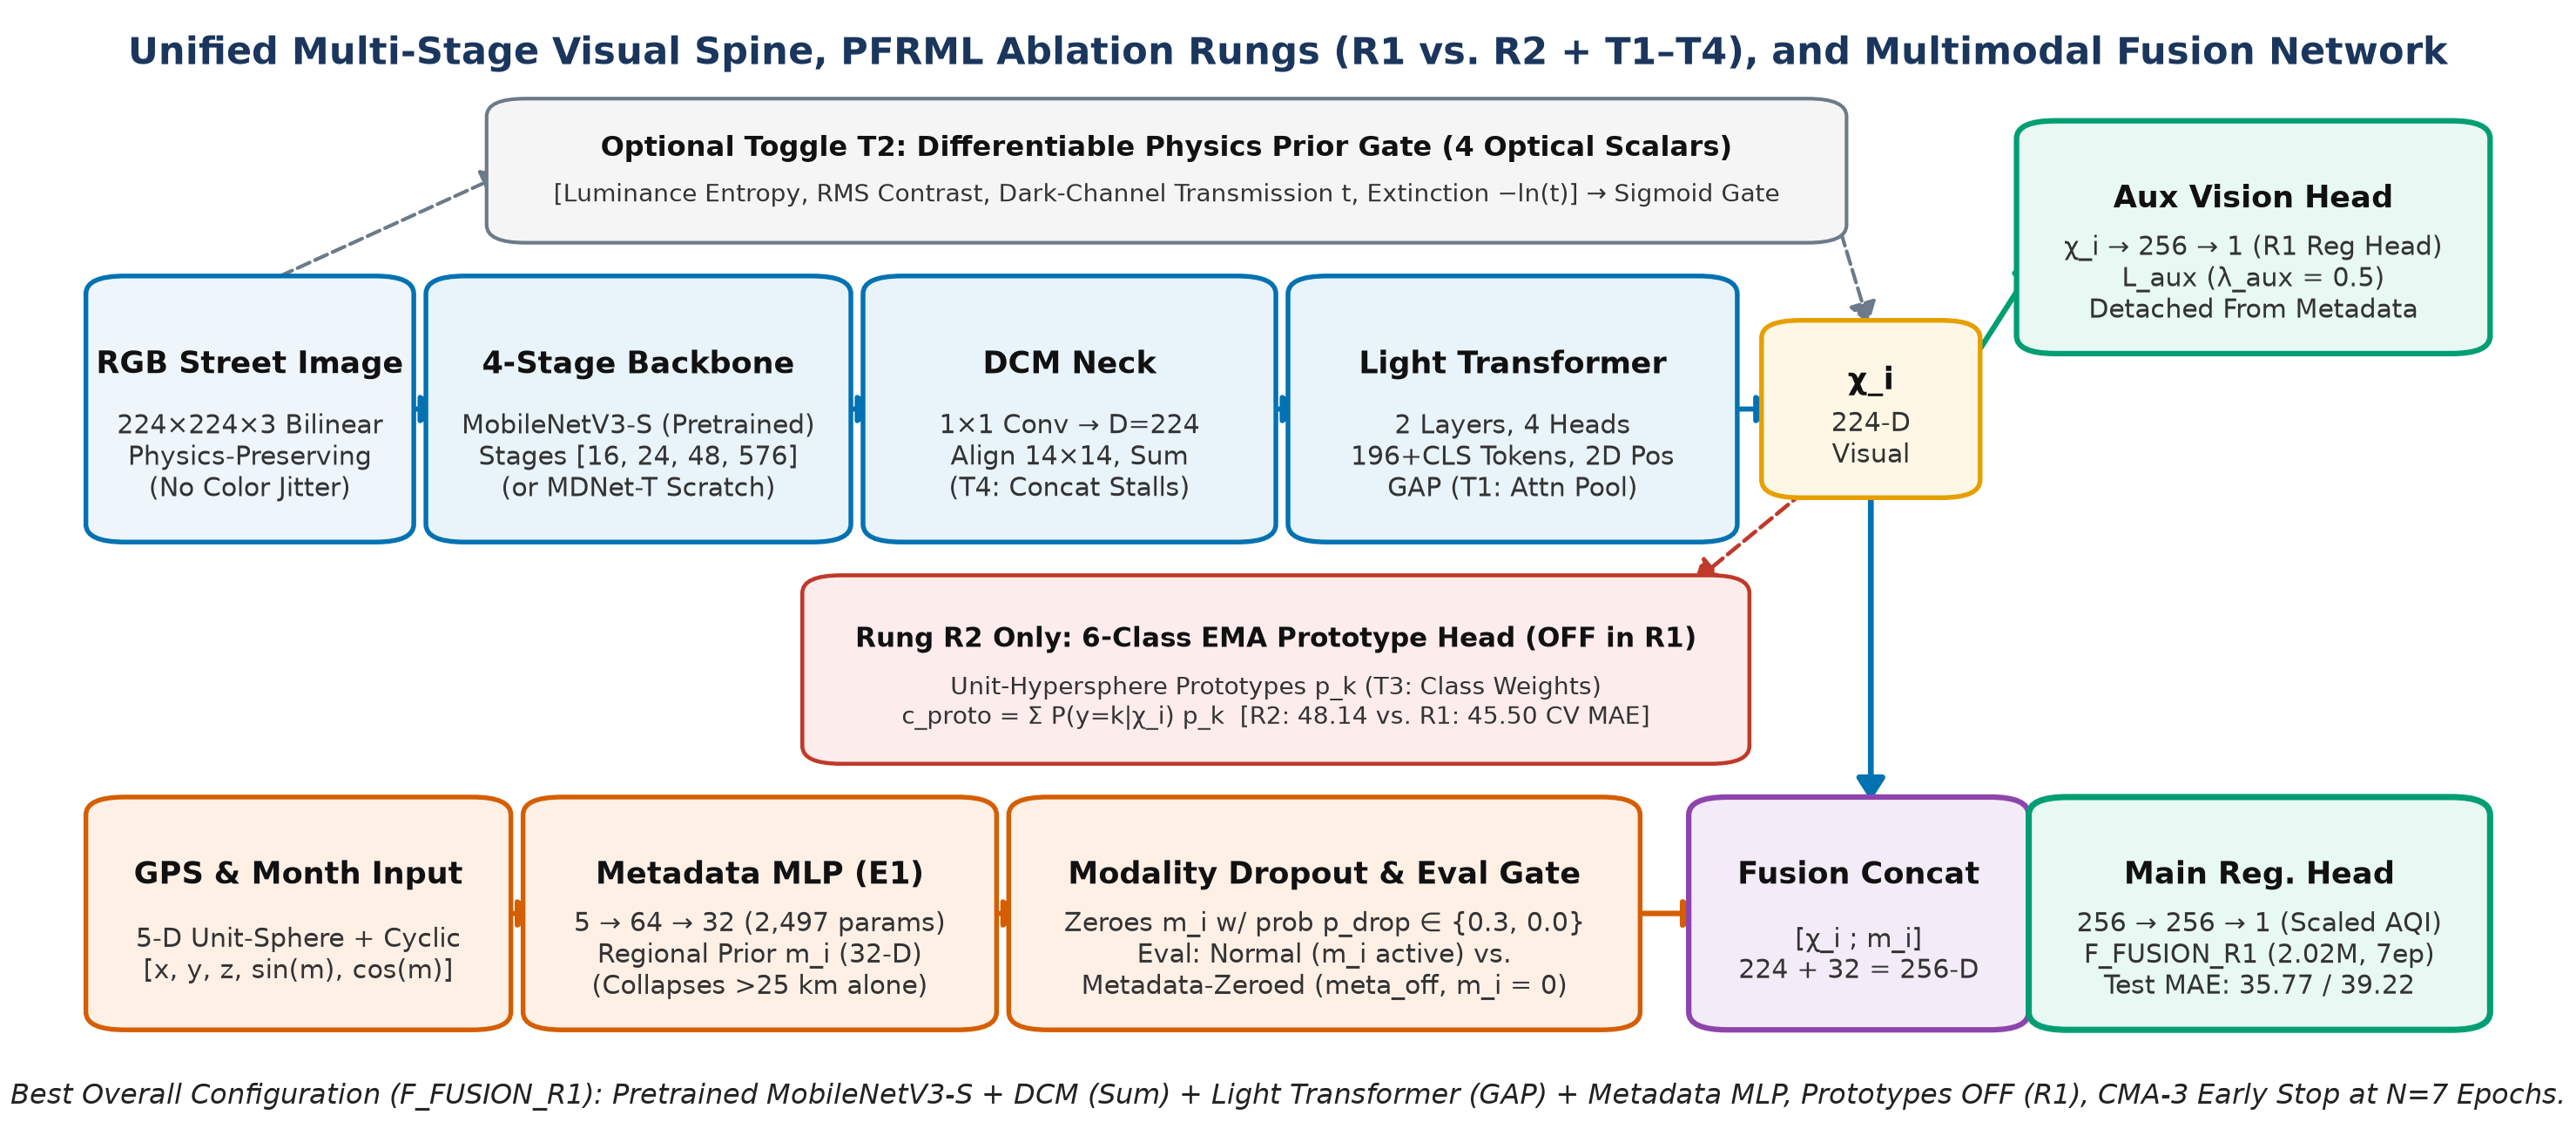
\includegraphics[width=0.98\textwidth]{figures/ieee_fig2_architecture.png}
  \caption{
    Unified architecture of the multi-stage DCM + Light Transformer visual
    spine, the R1/R2 prototype multitask heads and literature toggles (T1--T4),
    and the multimodal fusion network.
  }
  \label{fig:architecture}
\end{figure*}

\subsubsection{Dimension Consistency Module (DCM) and Light Transformer}

Given four hierarchical stage feature maps at spatial sizes $56 \times 56$,
$28 \times 28$, $14 \times 14$, and $7 \times 7$, the Dimension Consistency
Module projects each stage to $D = 224$ channels via a $1 \times 1$ convolution,
aligns every map to a $14 \times 14$ grid using static pooling or upsampling
($4 \times 4$ MaxPool for Stage~1, $2 \times 2$ MaxPool for Stage~2, Identity
for Stage~3, and $2 \times$ bilinear Upsample for Stage~4), applies 2D LayerNorm
and average pooling, and fuses the aligned maps. Following Table~I (DCM Stage~5)
of Wang et al.~\cite{wangPrototypeFeatureRepresentationGuided2026}, our default
fusion is element-wise summation, while Toggle~T4 tests channel concatenation
($896 \to 224$) followed by 2D LayerNorm.

Next, the Light Transformer Encoder flattens the $14 \times 14$ feature grid
into 196 spatial tokens, prepends a learnable \texttt{[CLS]} token to form 197
tokens of dimension 224, and adds a factored 2D learnable row-and-column
positional encoding. The sequence passes through a 2-layer pre-norm Transformer
encoder (4 attention heads, feed-forward width 448, GELU activation, dropout
0.1) and final LayerNorm. By default, the 196 encoded spatial tokens are
averaged via uniform Global Average Pooling into a single 224-D visual
representation $\chi_i$.

\subsubsection{
  Prototype Classification Head, EMA Updates, and the Eq.~5 vs.\ Fig.~7
  Regression Ambiguity
}

In the Prototype Classification Head, $K = 6$ class reference vectors
(prototypes) $\{p_k\}_{k=0}^5$ of dimension 224 are stored as persistent,
gradient-free buffers initialized orthogonally on the unit hypersphere. Both the
pooled image feature $\chi_i$ and the prototypes $p_k$ are $L_2$-normalized to
unit length, and class probabilities are assigned via temperature-scaled
negative squared Euclidean distance:
\begin{equation}
  P(y = k \mid \chi_i) = \frac{\exp\!\big( -\|\hat{\chi}_i - \hat{p}_k\|_2^2 / \tau \big)}{\sum_{j=0}^{5} \exp\!\big( -\|\hat{\chi}_i - \hat{p}_j\|_2^2 / \tau \big)}, \label{eq:proto_softmax}
\end{equation}
where $\tau > 0$ is a learnable temperature parameter initialized at 0.2. At the
end of warmup epoch~3, prototypes are re-initialized from the normalized class
centroids of the active training fold's features in evaluation mode; during
training batches, any class $k$ present in the mini-batch updates its prototype
without gradients via Exponential Moving Average (EMA) with decay 0.9 ($90\%$
previous prototype plus $10\%$ current batch centroid, re-normalized to unit
length).

While implementing the Prototype-Guided Regression Head, we identified a
structural ambiguity in the PFRML
paper~\cite{wangPrototypeFeatureRepresentationGuided2026}: Section~II-D (Eq.~5
and Fig.~5) writes the continuous regression MLP $h(\cdot)$ directly as a
function of the backbone feature $\chi_i$ in parallel with the prototype
classifier, whereas Section~III-C3 (Fig.~7) explicitly labels the full model
\textit{``w/ prototype (prototype-weighted feature)''} contrasted against
\textit{``w/o prototype''}. Rather than guessing which formulation performs
better, we implemented all three variants as explicit ablation rungs using a
single regression MLP
($\text{Linear}(D_{\text{in}}, 256) \to \text{GELU} \to \text{Dropout}(0.1) \to \text{Linear}(256, 1)$):
\begin{itemize}
  \item \textbf{Rung R1 (No Prototypes, ``w/o prototype''):} Removes the
        prototype head and classification loss completely, feeding $\chi_i$
        ($D_{\text{in}} = 224$) directly to the regression MLP under pure MSE
        loss (1.95M parameters).
  \item \textbf{Rung R2 (PFRML Baseline, \texttt{chi\_proto}, Fig.~7
        interpretation):} Computes the prototype-weighted feature
        $\tilde{c}_i = \sum_{k=0}^{5} P(y = k \mid \chi_i)\,\hat{p}_k$ and feeds
        the concatenated 448-D vector $[\chi_i; \tilde{c}_i]$ into the
        regression MLP (2.01M parameters).
  \item \textbf{Rung R2 Eq.~5 Literal (\texttt{reg\_input=chi}):} Feeds only
        $\chi_i$ ($D_{\text{in}} = 224$) into the regression MLP while keeping
        the prototype classification head and hybrid multitask loss active in
        parallel.
\end{itemize}

\subsubsection{Literature Toolbox Toggles (T1--T4)}

Onto the R2 baseline, we evaluate four individual architectural toggles and
their combination (R2+all):
\begin{itemize}
  \item \textbf{Toggle T1 -- Spatial Token Attention Pooling:} Inspired by
        SkyFuseNet~\cite{abdelsalamSkyFuseNetCrossAttentionSwin2026} (Sec.~III,
        Eq.~2) and GWAP~\cite{leeEnhancingPM25Detection2025} (Eq.~7), replaces
        uniform GAP over the 196 spatial tokens with a learnable linear-softmax
        spatial attention gate so the model can weight sky and horizon tokens
        above foreground pavement.
  \item \textbf{Toggle T2 -- Differentiable Physics Prior Gate:} Inspired by
        Doha et al.~\cite{dohaDeepMultiTaskLearning2026} (Sec.~3.3 \& 3.5,
        Eq.~9) and Yadav et al.~\cite{yadavRoadsideTreeImageBased2025}
        (Sec.~IV), computes four global atmospheric physics scalars inside the
        forward pass on unnormalized $[0,1]$ RGB pixels: soft-histogram Shannon
        entropy of luminance, root-mean-square luminance contrast, mean
        dark-channel transmission $t$, and optical extinction $-\ln(t)$. A
        linear layer projects these 4 scalars to 224 dimensions, and a learned
        channel-wise sigmoid gate blends the physics projection with the deep
        visual feature $\chi_i$.
  \item \textbf{Toggle T3 -- Fold-Internal Inverse-Frequency Class Weights:}
        Following Doha et al.~\cite{dohaDeepMultiTaskLearning2026} (Eq.~11),
        Byler et al.~\cite{bylerLocationGeneralizabilityImageBased2025}
        (Sec.~4.1), and Mohan et al.~\cite{mohanDeepLearningBasedPM252025},
        weights each class $k$ in the cross-entropy loss by dampened inverse
        class frequency ($N_k^{-0.5}$, normalized to unit mean) computed
        \textit{strictly from the active training fold's class counts} $N_k$,
        up-weighting rare \textit{Very Unhealthy} and \textit{Hazardous}
        samples.
  \item \textbf{Toggle T4 -- DCM Concatenation:} Replaces element-wise summation
        in the DCM with 4-stage channel concatenation ($896 \to 224$) and 2D
        LayerNorm.
  \item \textbf{Combined R2+all:} Combines R2 with all three approved toggles
        (T1 attention pooling + T2 physics prior gate + T3 class weights) while
        retaining default element-wise summation in the DCM (2.11M parameters).
\end{itemize}

\subsection{
  Multimodal Fusion, Modality Dropout, Vision Auxiliary Loss, and Early Stopping
  (E5)
}
\label{subsec:fusion_methodology}

To address RQ4, our Multimodal Fusion Model combines the visual spine with the
5-input Metadata MLP encoder (which maps GPS and month into a 32-D embedding
$m_i$). We evaluate both the prototype-free R1 visual neck (2.02M parameters,
where the main regression MLP reads $[\chi_i; m_i]$ of dimension
$256 \to 256 \to 1$) and the full PFRML visual neck (2.18M parameters, where the
prototype classifier operates strictly on visual features $\chi_i$ and the
regression MLP reads $[\chi_i; \tilde{c}_i; m_i]$ of dimension
$480 \to 256 \to 1$).

Because the low-dimensional metadata branch $m_i$ converges much faster than the
deep visual backbone, naive joint training risks ignoring the image entirely. We
incorporate three mechanisms under 5-fold 25~km spatial-cluster CV:
\begin{enumerate}
  \item \textbf{Per-sample Modality Dropout ($p_{\text{drop}}$):} During
        training, for each sample in a mini-batch independently, the 32-D
        metadata embedding $m_i$ is zeroed out with probability
        $p_{\text{drop}} \in \{0.3, 0.0\}$, forcing the shared regression head
        to practice predicting AQI from $\chi_i$ alone.
  \item \textbf{Detached Auxiliary Vision-Only Regression Head:} A separate
        auxiliary regression MLP ($224 \to 256 \to 1$) predicts scaled AQI
        strictly from the visual feature $\chi_i$. Combined with the PFRML
        hybrid objective, the general training loss is:
        \begin{equation}
          \mathcal{L}
          = \mathcal{L}_{\text{cls}}
            + \beta\,\mathcal{L}_{\text{reg}}
            + \lambda_{\text{aux}}\,\mathcal{L}_{\text{aux}}, \label{eq:total_loss}
        \end{equation}
        where $\mathcal{L}_{\text{cls}}$ is label-smoothing cross-entropy
        ($\epsilon = 0.1$; zero in R1 when prototypes are disabled),
        $\mathcal{L}_{\text{reg}}$ is main regression MSE ($\beta = 0.5$ when
        prototypes are active, $1.0$ in R1), and $\mathcal{L}_{\text{aux}}$ is
        auxiliary vision-only MSE weighted by $\lambda_{\text{aux}} = 0.5$
        (active in fusion models, with gradients flowing into the visual spine
        and detached from the Metadata MLP).
  \item \textbf{Metadata-Zeroed Diagnostic Evaluation (\texttt{meta\_off}) and
        CMA-3 Early-Stopping Selection:} Every trained fusion checkpoint is
        evaluated twice: normally ($m_i$ active) and with metadata zeroed out at
        test time ($m_i = 0$) to measure how well the joint regression head
        performs when deprived of location cues. Furthermore, because 30-epoch
        fusion models progressively overfit training cluster coordinates after
        the first few epochs, we implemented a pre-committed epoch-selection
        protocol: across the 5-fold spatial-cluster validation curves of the
        30-epoch R1 fusion run ($p_{\text{drop}} = 0.0$), we computed the
        3-epoch centered moving average (CMA-3, averaging epochs $t - 1$, $t$,
        and $t + 1$) of the 5-fold mean validation MAE for $t \ge 6$. Minimizing
        CMA-3 selected epoch $N = 7$ ($\text{CMA-3} = 46.26$, raw 5-fold mean
        $\text{MAE} = 45.74 \pm 6.78$). We then trained a fresh 5-fold
        spatial-cluster CV run with a 7-epoch cosine schedule under a
        pre-committed decision rule: adopt $E_{\text{final}} = 7$ epochs for
        final one-shot test evaluation if and only if its 5-fold last-epoch mean
        MAE beat $46.95$ (the 30-epoch baseline $47.45$ minus a $0.50$ margin).
        It achieved $44.40 \pm 7.30 < 46.95$, locking in $E_{\text{final}} = 7$
        for our final fusion model \texttt{F\_FUSION\_R1}.
\end{enumerate}

\section{Results}
\label{sec:results}

All cross-validation results reported in this section are authoritative
\textbf{last-epoch} metrics verified from the repository's tracked
\texttt{REPORT\_NUMBERS.md} report (Sections 2--7), and all final one-shot test
results and 95\% station-level cluster bootstrap confidence intervals are
verified from \texttt{REPORT\_NUMBERS.md} (Section~6) and
\texttt{final\_comparison.md}.

\subsection{Non-Visual Baselines and the Geospatial Shortcut (E0, E1)}
\label{subsec:results_baselines}

\begin{table*}[t]
  \centering
  \caption{
    Non-Visual and Handcrafted Optical Baselines Across 5-Fold Station CV
    ($n = 8,176$), 5-Fold 25~km Spatial-Cluster CV ($n = 8,176$), Full Test Set
    ($n = 2,920$, 729 Stations), and Unseen-Region Test Subset ($> 25$~km,
    $n = 717$, 205 Stations). MAE Reports 5-Fold Mean $\pm$ SD or Test Point
    Estimate [95\% Station-Bootstrap CI].
  }
  \label{tab:baselines}
  \footnotesize
  \setlength{\tabcolsep}{4.5pt}
  \resizebox{\textwidth}{!}{%
    \begin{tabular}{llccccccccccc}
      \toprule
      \textbf{Baseline Model (ID)}                 & \textbf{Evaluation Split} & $\boldsymbol{n}$ & \textbf{MAE (Mean $\pm$ SD / [95\% CI])} & \textbf{RMSE} & \textbf{PLCC} & \textbf{SRCC} & $\boldsymbol{R^2}$ & \textbf{Acc} & $\boldsymbol{\pm 1}$\textbf{Acc} & \textbf{MacroF1} & \textbf{TailMAE} & \textbf{TailF1} \\
      \midrule
      Constant Median (\texttt{E0\_median})        & Station 5-fold CV         &       8176       &             $66.21 \pm 4.89$             &    $88.23$    &   $0.0000$    &   $0.0000$    &     $-0.0161$      &   $0.2153$   &             $0.6497$             &     $0.0590$     &     $176.95$     &    $0.0000$     \\
      Constant Median (\texttt{E0\_median})        & Spatial-Cluster 5-fold CV &       8176       &             $66.14 \pm 5.60$             &    $88.00$    &   $0.0000$    &   $0.0000$    &     $-0.0168$      &   $0.2154$   &             $0.6500$             &     $0.0591$     &     $175.81$     &    $0.0000$     \\
      Constant Median (\texttt{E0\_median})        & Full Test Set             &       2920       &                 $63.64$                  &    $81.88$    &   $0.0000$    &   $0.0000$    &     $-0.0105$      &   $0.2158$   &             $0.6473$             &     $0.0592$     &     $155.88$     &    $0.0000$     \\
      Constant Median (\texttt{E0\_median})        & Test $> 25$~km Subset     &       717        &                 $56.60$                  &    $64.22$    &   $0.0000$    &   $0.0000$    &     $-0.0049$      &   $0.2022$   &             $0.6318$             &     $0.0561$     &     $102.78$     &    $0.0000$     \\
      \midrule
      Haze-Stats Ridge (\texttt{E0\_ridge})        & Station 5-fold CV         &       8176       &             $64.11 \pm 4.40$             &    $86.32$    &   $0.1998$    &   $0.2354$    &      $0.0301$      &   $0.2450$   &             $0.6925$             &     $0.1330$     &     $158.15$     &    $0.0000$     \\
      Haze-Stats Ridge (\texttt{E0\_ridge})        & Spatial-Cluster 5-fold CV &       8176       &             $64.56 \pm 5.02$             &    $87.37$    &   $0.1526$    &   $0.1982$    &     $-0.0018$      &   $0.2415$   &             $0.6915$             &     $0.1325$     &     $160.68$     &    $0.0000$     \\
      Haze-Stats Ridge (\texttt{E0\_ridge})        & Full Test Set             &       2920       &                 $60.84$                  &    $79.77$    &   $0.2112$    &   $0.2258$    &      $0.0408$      &   $0.2250$   &             $0.6815$             &     $0.1109$     &     $140.91$     &    $0.0000$     \\
      Haze-Stats Ridge (\texttt{E0\_ridge})        & Test $> 25$~km Subset     &       717        &                 $53.76$                  &    $65.26$    &   $0.1435$    &   $0.0970$    &     $-0.0377$      &   $0.2092$   &             $0.6792$             &     $0.1142$     &     $107.93$     &    $0.0000$     \\
      \midrule
      GPS + Month MLP (\texttt{E1\_metadata\_mlp}) & Station 5-fold CV         &       8176       &        $\mathbf{43.15 \pm 7.47}$         &    $65.43$    &   $0.6704$    &   $0.7260$    &      $0.4438$      &   $0.4234$   &             $0.8794$             &     $0.3506$     &     $104.96$     &    $0.1632$     \\
      GPS + Month MLP (\texttt{E1\_metadata\_mlp}) & Spatial-Cluster 5-fold CV &       8176       &        $\mathbf{46.00 \pm 7.33}$         &    $70.09$    &   $0.6257$    &   $0.7147$    &      $0.3647$      &   $0.4183$   &             $0.8603$             &     $0.3556$     &     $118.49$     &    $0.1953$     \\
      GPS + Month MLP (\texttt{E1\_metadata\_mlp}) & Full Test Set             &       2920       &     $\mathbf{40.34}\;[34.45, 48.31]$     &    $57.70$    &   $0.7098$    &   $0.7344$    &      $0.4982$      &   $0.4096$   &             $0.8873$             &     $0.3397$     &     $76.82$      &    $0.1362$     \\
      GPS + Month MLP (\texttt{E1\_metadata\_mlp}) & Test $> 25$~km Subset     &       717        &     $\mathbf{49.84}\;[40.18, 58.81]$     &    $65.31$    &   $0.3797$    &   $0.4954$    & $\mathbf{-0.0393}$ &   $0.2929$   &             $0.7476$             &     $0.2004$     &     $88.83$      &    $0.0000$     \\
      \bottomrule
    \end{tabular}%
  }
\end{table*}

Table~\ref{tab:baselines} answers RQ1 by exposing both the weakness of shallow
handcrafted haze statistics on heterogeneous global street imagery and the
strength---and fragility---of the geospatial shortcut:
\begin{enumerate}
  \item \textbf{Handcrafted haze statistics barely improve over trivial
        guessing:} Haze-Statistics Ridge Regression (\texttt{E0\_ridge}) reduces
        5-fold station CV MAE by only 2.10 points over the Constant Median
        Predictor ($64.11 \pm 4.40$ vs.\ $66.21 \pm 4.89$, $R^2 = 0.0301$,
        $\text{PLCC} = 0.1998$) and by 2.80 points on the full test set ($60.84$
        vs.\ $63.64$, $R^2 = 0.0408$). On unconstrained global street scenes
        where sky fraction, building textures, and illumination vary widely
        across cameras, linear combinations of global/half-image HSV saturation,
        Sobel contrast, and Dark Channel statistics carry minimal predictive
        power.
  \item \textbf{The geospatial shortcut illusion and its collapse beyond 25~km:}
        Without examining a single image pixel, the 2,497-parameter Metadata MLP
        (\texttt{E1\_metadata\_mlp}) achieves $43.15 \pm 7.47$ MAE
        ($R^2 = 0.4438$, $\text{SRCC} = 0.7260$) in station CV and
        \textbf{40.34~[34.45, 48.31] MAE} ($R^2 = 0.4982$,
        $\pm 1\text{Acc} = 0.8873$) on the full test set. However, when nearby
        same-city stations are grouped into 25~km clusters (spatial-cluster CV),
        Metadata MLP degrades to $46.00 \pm 7.33$ MAE ($R^2 = 0.3647$, with
        Fold~0 jumping from 39.71 to 55.86). Most importantly, on the
        unseen-region test subset \texttt{test\_gt25km} ($n = 717$, 205 stations
        $> 25$~km from any training station), Metadata MLP jumps by $+9.50$ MAE
        points to \textbf{49.84~[40.18, 58.81]}, while its explained variance
        collapses to \textbf{$R^2 = -0.0393$} (worse than predicting the
        constant subset mean), 6-class accuracy drops from 0.4096 to 0.2929, and
        TailF1 falls to 0.0000.
\end{enumerate}

\subsection{
  Image-Only Backbones: Transfer Learning vs.\ From-Scratch Dilated CNNs (E2,
  E3, E3b)
}
\label{subsec:results_backbones}

\begin{table*}[t]
  \centering
  \caption{
    Image-Only Backbones Under 5-Fold Station-Grouped Cross-Validation
    ($n = 8,176$, Authoritative Last-Epoch Metrics). Skill Is Computed Relative
    to the Constant Median Baseline (Station CV MAE $= 66.21$).
  }
  \label{tab:image_backbones}
  \footnotesize
  \setlength{\tabcolsep}{4pt}
  \resizebox{\textwidth}{!}{%
    \begin{tabular}{llcccccccccccc}
      \toprule
      \textbf{Vision Model (ID)}             & \textbf{Params / Schedule} &   \textbf{Last-Ep MAE}    &   \textbf{Skill}   &  \textbf{F0 / F1 / F2 / F3 / F4 MAE}  &  \textbf{RMSE}   &   \textbf{PLCC}   &   \textbf{SRCC}   & $\boldsymbol{R^2}$ &   \textbf{Acc}    & $\boldsymbol{\pm 1}$\textbf{Acc} & \textbf{MacroF1}  & \textbf{TailMAE}  &  \textbf{TailF1}  \\
      \midrule
      ResNet-18 Pretrained (\texttt{E2})     & 11.18M (lr 3e-4, 40ep)     & $\mathbf{44.05 \pm 8.70}$ & $\mathbf{+0.3346}$ & 34.85 / 43.35 / 42.06 / 58.45 / 41.55 & $\mathbf{68.22}$ & $\mathbf{0.6441}$ & $\mathbf{0.7060}$ & $\mathbf{0.3862}$  &     $0.4102$      &        $\mathbf{0.8656}$         &     $0.3751$      & $\mathbf{116.26}$ &     $0.2822$      \\
      MobileNetV3-S + MD-Neck (\texttt{E3b}) & 1.04M (lr 1e-3, 40ep)      & $\mathbf{44.92 \pm 8.54}$ &     $+0.3214$      & 34.51 / 45.40 / 43.31 / 58.25 / 43.14 &     $70.23$      &     $0.6173$      &     $0.6780$      &      $0.3461$      & $\mathbf{0.4137}$ &             $0.8482$             & $\mathbf{0.3789}$ &     $118.93$      &     $0.2913$      \\
      MobileNetV3-S Pretrained (\texttt{E2}) & 1.52M (lr 1e-3, 30ep)      & $\mathbf{45.66 \pm 8.41}$ &     $+0.3103$      & 36.27 / 46.10 / 42.96 / 59.21 / 43.77 &     $70.41$      &     $0.6152$      &     $0.6695$      &      $0.3450$      &     $0.4044$      &             $0.8488$             &     $0.3776$      &     $119.16$      & $\mathbf{0.3135}$ \\
      \midrule
      ResNet-18 Scratch (\texttt{E2})        & 11.18M (lr 1e-3, 30ep)     &     $53.27 \pm 7.11$      &     $+0.1954$      & 48.41 / 50.21 / 53.62 / 65.44 / 48.67 &     $76.77$      &     $0.5177$      &     $0.5367$      &      $0.2314$      &     $0.3276$      &             $0.7943$             &     $0.2975$      &     $126.93$      &     $0.2302$      \\
      Paper 2 MDNet-T Scratch (\texttt{E3})  & 4.93M (lr 1e-3, 60ep)      &     $53.29 \pm 6.38$      &     $+0.1951$      & 48.37 / 50.74 / 53.97 / 64.06 / 49.31 &     $77.16$      &     $0.5260$      &     $0.5365$      &      $0.2226$      &     $0.3371$      &             $0.7797$             &     $0.3030$      &     $129.51$      &     $0.2175$      \\
      \bottomrule
    \end{tabular}%
  }
\end{table*}

During Stage~1/2 Fold-0 hyperparameter screening (1-fold screens, never quoted
as 5-fold CV results), tuning pretrained ResNet-18 to
$\text{lr} = 3 \times 10^{-4}$ for 40 epochs improved Fold-0 last-epoch MAE from
40.28 to 34.85, extending from-scratch MDNet-T from 30 to 60 epochs improved
Fold-0 MAE from 51.58 (vs.\ 52.50 for 6-class classification MDNet-T) to 48.37,
and running our MobileNetV3-S + MD-Neck adaptation at $\text{lr} = 10^{-3}$ for
40 epochs achieved 34.51 on Fold~0 (vs.\ 35.66 at
$\text{lr} = 3 \times 10^{-4}$). By contrast, screening pretrained
MobileNetV3-Small at $\text{lr} = 3 \times 10^{-4}$ (40.15) and from-scratch
ResNet-18 at 60 epochs (48.48) did not meet the 1.0-MAE promotion threshold over
their 30-epoch defaults (36.27 and 48.41).

Table~\ref{tab:image_backbones} presents the full 5-fold station CV results for
the five promoted vision families, yielding three answers to RQ2 (see
Fig.~\ref{fig:backbones_fold3}):
\begin{enumerate}
  \item \textbf{ImageNet pretraining is the single largest visual lever ($-7.61$
        to $-9.24$ MAE):} All three ImageNet-pretrained models---ResNet-18
        Pretrained ($44.05 \pm 8.70$, $\text{Skill} = +0.3346$), our adaptation
        MobileNetV3-S + MD-Neck ($44.92 \pm 8.54$, $\text{Skill} = +0.3214$),
        and plain MobileNetV3-Small Pretrained ($45.66 \pm 8.41$,
        $\text{Skill} = +0.3103$)---outperform both from-scratch networks
        (ResNet-18 Scratch at $53.27 \pm 7.11$ and Paper~2's MDNet-T Scratch at
        $53.29 \pm 6.38$) by roughly 8--9 MAE points on every single fold, while
        lifting SRCC from $\sim 0.537$ to $0.670\text{--}0.706$ and $R^2$ from
        $0.22\text{--}0.23$ to $0.35\text{--}0.39$.
  \item \textbf{From-scratch MDNet-T ties from-scratch ResNet-18:} Despite its
        theoretical 1,136-pixel multiscale dilated receptive field and 60
        training epochs, from-scratch MDNet-T ($53.29 \pm 6.38$) matches
        from-scratch ResNet-18 ($53.27 \pm 7.11$). On roughly 6,540
        heterogeneous training images per fold, random initialization lacks the
        generic edge, sky, and depth representations provided by ImageNet
        pretraining.
  \item \textbf{Our MobileNetV3-S + MD-Neck adaptation (\texttt{E3b}) and plain
        MobileNetV3-Small closely match ResNet-18:} Adding two MDBlock(128)
        layers onto pretrained MobileNetV3-Small (\texttt{E3b}, 1.04M
        parameters) lowers 5-fold mean MAE slightly from 45.66 to 44.92 and
        achieves the highest 6-class accuracy (0.4137) and Macro-F1 (0.3789)
        among image baselines, while plain MobileNetV3-Small (1.52M parameters)
        achieves the highest TailF1 (0.3135) and trains in 15--22~s/epoch at
        roughly $7 \times$ fewer parameters than ResNet-18 (11.18M). All three
        pretrained backbones cluster within 1.61 MAE points (well within the
        cross-fold standard deviation of $\sim 8.5$ points), motivating
        pretrained MobileNetV3-Small as the fast visual backbone for our 5-fold
        PFRML ablation ladder.
\end{enumerate}

\begin{figure}[t]
  \centering
  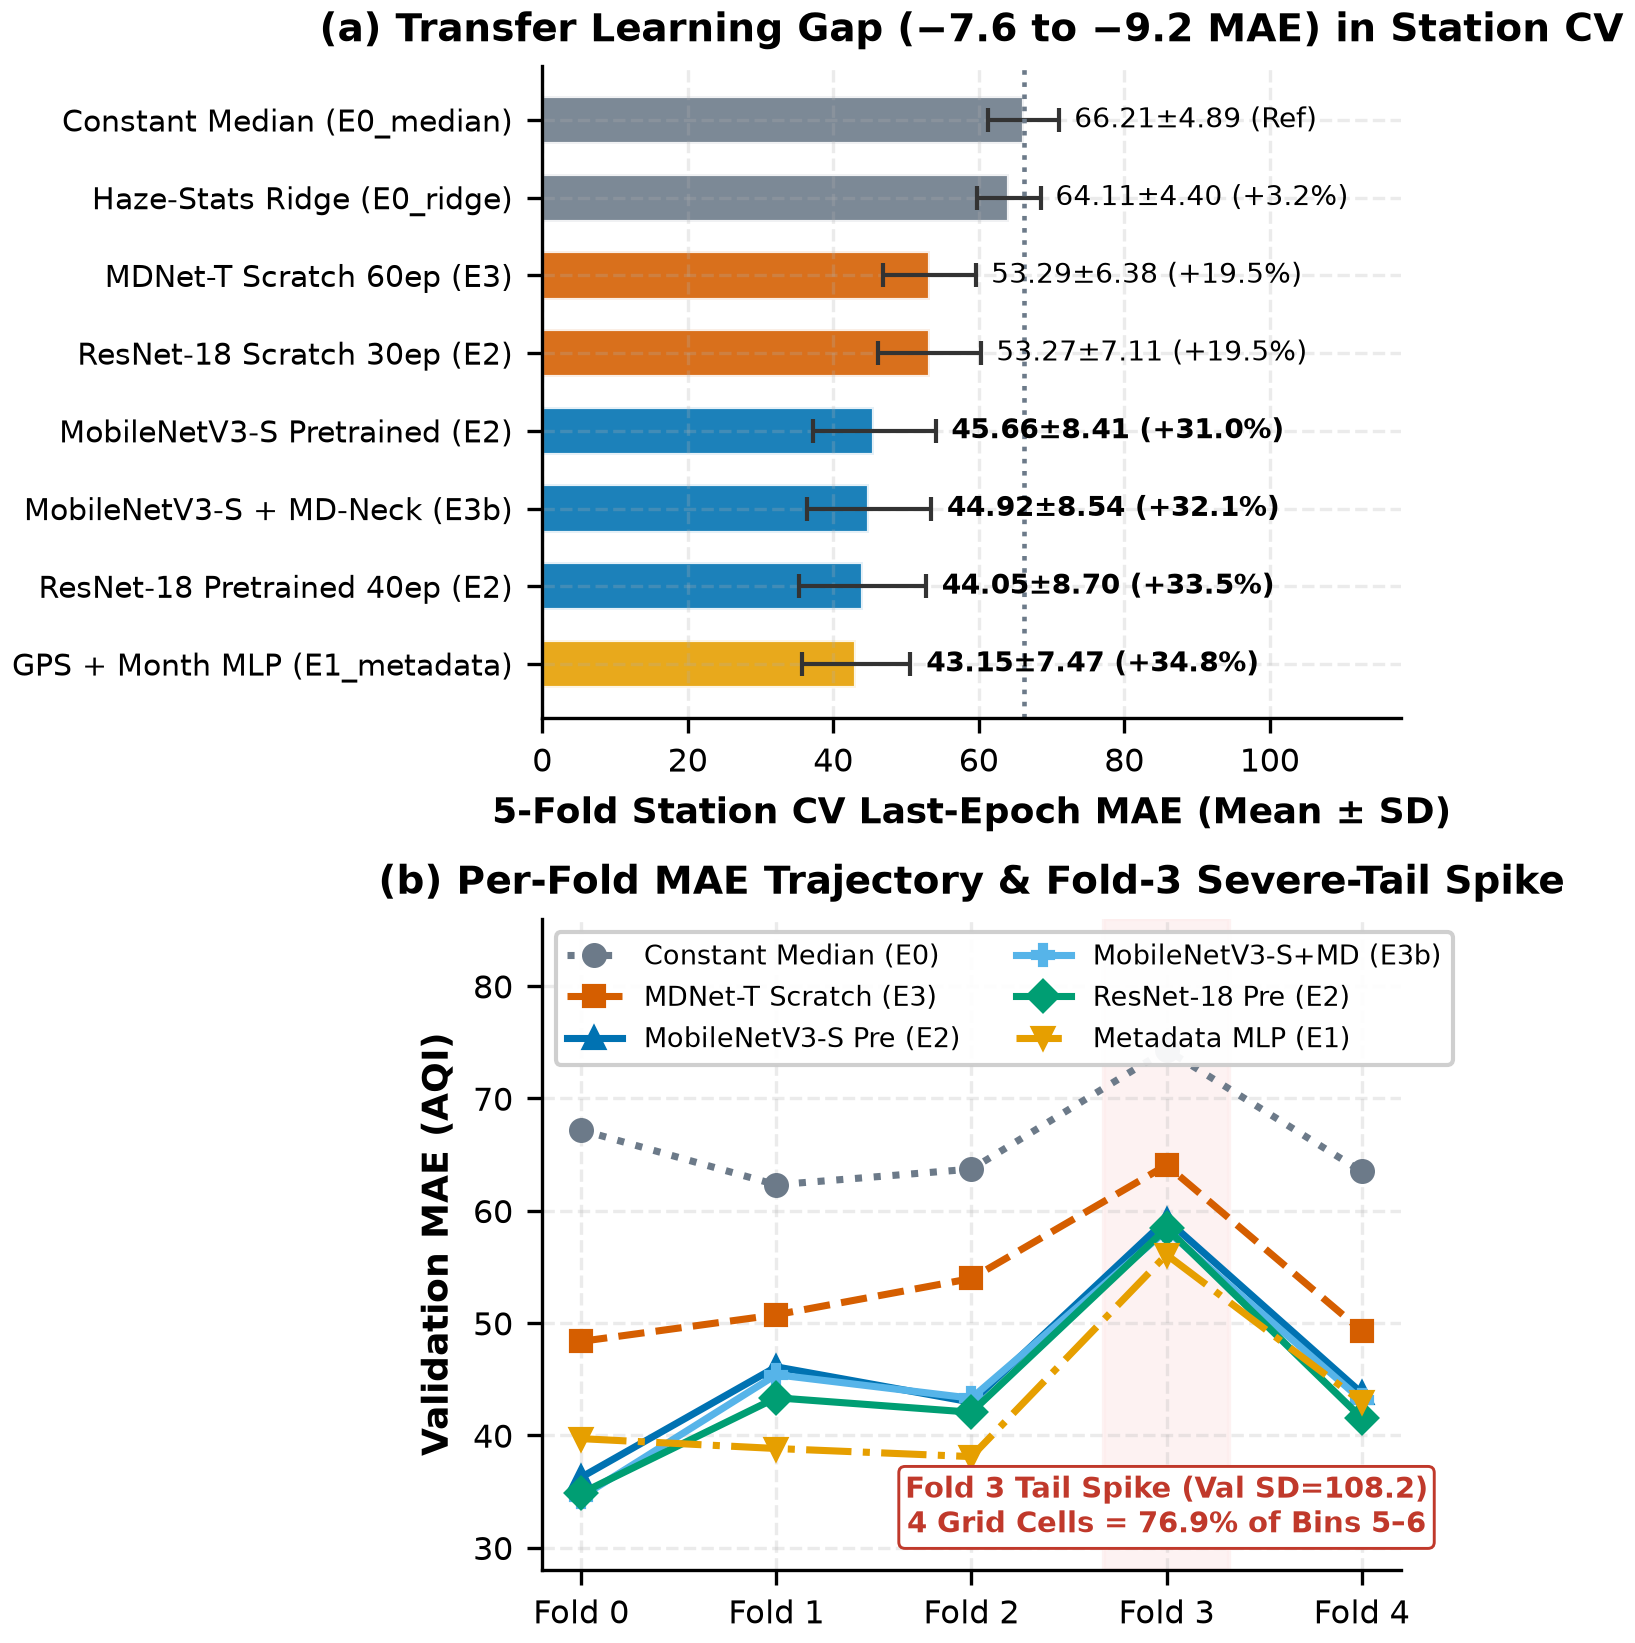
\includegraphics[width=\columnwidth]{figures/ieee_fig3_backbones_fold3.png}
  \caption{
    Image-only backbone comparison showing the 7.6--9.2 MAE transfer-learning
    gain and uniform Fold~3 tail sensitivity across all models.
  }
  \label{fig:backbones_fold3}
\end{figure}

\subsection{
  PFRML 5-Fold Ablation Ladder: Why Prototypes Degrade Global Regression (E4,
  E5)
}
\label{subsec:results_pfrml}

\begin{table*}[t]
  \centering
  \caption{
    PFRML 5-Fold Station-Grouped CV Ablation Ladder ($n = 8,176$, Authoritative
    Last-Epoch Metrics). Paired Differences Report Mean Difference $\pm$
    Standard Error (Candidate Minus Reference; Negative Means Candidate Lowers
    MAE) and Folds Won Out of 5.
  }
  \label{tab:pfrml_ablation}
  \footnotesize
  \setlength{\tabcolsep}{4pt}
  \resizebox{\textwidth}{!}{%
    \begin{tabular}{lccccccccccc}
      \toprule
      \textbf{Ablation Rung / Configuration}                             &   \textbf{Last-Ep MAE}    &   \textbf{Skill}   & \textbf{Diff vs.\ R1 (Won)} & \textbf{Diff vs.\ E2 (Won)} &       \textbf{Diff vs.\ R2 (Won)}        &  \textbf{RMSE}   &   \textbf{SRCC}   & $\boldsymbol{R^2}$ &   \textbf{Acc}    & $\boldsymbol{\pm 1}$\textbf{Acc} & \textbf{TailMAE}  \\
      \midrule
      \textbf{R1:} DCM + Transformer + MLP (No Prototypes)               & $\mathbf{45.50 \pm 8.64}$ & $\mathbf{+0.3127}$ &   $+0.00 \pm 0.00$ (---)    &   $-0.16 \pm 0.36$ (4/5)    & $\mathbf{-2.63 \pm 1.10}$ (\textbf{4/5}) & $\mathbf{71.44}$ & $\mathbf{0.6671}$ & $\mathbf{0.3249}$  &     $0.4080$      &        $\mathbf{0.8448}$         & $\mathbf{115.37}$ \\
      \textbf{R2:} PFRML Baseline (\texttt{chi\_proto}, toggles off)     &     $48.14 \pm 7.61$      &     $+0.2729$      &   $+2.63 \pm 1.10$ (1/5)    &   $+2.47 \pm 0.95$ (1/5)    &          $+0.00 \pm 0.00$ (---)          &     $75.43$      &     $0.6327$      &      $0.2424$      &     $0.4088$      &             $0.8181$             &     $124.19$      \\
      \textbf{R2 Eq.~5:} Core PFRML (\texttt{reg\_input=chi}, CE active) &     $48.04 \pm 8.20$      &     $+0.2743$      &   $+2.54 \pm 0.42$ (0/5)    &   $+2.38 \pm 0.46$ (0/5)    &          $-0.09 \pm 0.73$ (2/5)          &     $75.14$      &     $0.6406$      &      $0.2538$      &     $0.4025$      &             $0.8182$             &     $123.27$      \\
      \midrule
      \textbf{R2 + T1:} Spatial Token Attention Pooling                  &     $48.40 \pm 7.74$      &     $+0.2689$      &   $+2.90 \pm 1.01$ (1/5)    &   $+2.74 \pm 0.97$ (1/5)    &          $+0.27 \pm 0.32$ (2/5)          &     $75.42$      &     $0.6352$      &      $0.2429$      &     $0.4032$      &             $0.8148$             &     $121.92$      \\
      \textbf{R2 + T2:} 4-Scalar Physics Prior Gate                      &     $47.57 \pm 6.73$      &     $+0.2815$      &   $+2.07 \pm 1.00$ (1/5)    &   $+1.91 \pm 0.78$ (1/5)    &          $-0.57 \pm 0.86$ (4/5)          &     $74.19$      &     $0.6405$      &      $0.2761$      &     $0.4037$      &             $0.8243$             &     $118.49$      \\
      \textbf{R2 + T3:} Fold-Internal Class Weights                      &     $47.06 \pm 8.01$      &     $+0.2892$      &   $+1.55 \pm 0.73$ (1/5)    &   $+1.40 \pm 0.50$ (0/5)    & $\mathbf{-1.08 \pm 0.49}$ (\textbf{4/5}) &     $73.67$      &     $0.6342$      &      $0.2822$      &     $0.4113$      &             $0.8142$             &     $124.33$      \\
      \textbf{R2 + T4:} DCM Concatenation (\textit{Failed})              &     $60.51 \pm 5.41$      &     $+0.0860$      &   $+15.01 \pm 3.38$ (0/5)   &   $+14.85 \pm 3.28$ (0/5)   &         $+12.38 \pm 3.49$ (0/5)          &     $85.22$      &     $0.4082$      &      $0.0556$      &     $0.3041$      &             $0.6664$             &     $168.58$      \\
      \textbf{R2 + all:} PFRML Full (T1 + T2 + T3, sum DCM)              &     $47.16 \pm 7.15$      &     $+0.2878$      &   $+1.65 \pm 0.92$ (2/5)    &   $+1.49 \pm 0.65$ (1/5)    &          $-0.98 \pm 0.90$ (4/5)          &     $74.22$      &     $0.6398$      &      $0.2774$      & $\mathbf{0.4150}$ &             $0.8136$             &     $121.05$      \\
      \midrule
      \textbf{Extra B:} PFRML on MDNet-T Scratch (\textit{Collapsed})    &     $66.56 \pm 4.88$      &     $-0.0053$      &   $+21.05 \pm 2.97$ (0/5)   &   $+20.90 \pm 2.79$ (0/5)   &         $+18.42 \pm 2.95$ (0/5)          &     $87.26$      &     $0.0817$      &      $0.0054$      &     $0.1489$      &             $0.4432$             &     $166.28$      \\
      \bottomrule
    \end{tabular}%
  }
\end{table*}

Table~\ref{tab:pfrml_ablation} presents the complete 5-fold station CV ablation
ladder for RQ3, yielding three decisive empirical findings:
\begin{enumerate}
  \item \textbf{The multi-stage DCM + Transformer neck without prototypes (R1)
        matches or slightly edges out the plain backbone:} R1 achieves
        \textbf{45.50 $\pm$ 8.64 MAE} ($\text{Skill} = +0.3127$, per-fold MAEs:
        35.71, 47.22, 41.94, 59.05, 43.59), beating plain pretrained
        MobileNetV3-Small (\texttt{E2}, $45.66 \pm 8.41$) on 4/5 folds (paired
        difference $-0.16 \pm 0.36$) while lowering TailMAE from 119.16 to
        115.37 and lifting TailF1 from 0.3135 to 0.3280.
  \item \textbf{Enabling the 6-class prototype multitask head (R2) consistently
        degrades continuous regression by 2.54 to 2.63 MAE points:} Turning on
        EMA prototypes and the hybrid multitask loss in R2 worsens 5-fold MAE to
        \textbf{48.14 $\pm$ 7.61} (paired difference $+2.63 \pm 1.10$ vs.\ R1,
        losing 4/5 folds; $+2.47 \pm 0.95$ vs.\ E2, losing 4/5 folds; $R^2$
        drops from 0.3249 to 0.2424). Furthermore, testing the literal Eq.~5
        variant (\texttt{reg\_input=chi}, where the regression MLP reads
        $\chi_i$ alone without concatenating $\tilde{c}_i$) yields virtually the
        exact same degraded performance: \textbf{48.04 $\pm$ 8.20 MAE} (paired
        difference $-0.09 \pm 0.73$ vs.\ R2; $+2.54 \pm 0.42$ vs.\ R1, losing
        \textbf{5/5 folds} to both R1 and E2). This proves that the Eq.~5
        vs.\ Fig.~7 ambiguity in Wang et
        al.~\cite{wangPrototypeFeatureRepresentationGuided2026} is not
        responsible for the drop; rather, imposing the 6-class prototype
        cross-entropy loss itself impairs continuous regression on global street
        imagery.
  \item \textbf{Literature toolbox toggles (T1--T3) provide at most $\sim 1.0$
        MAE recovery over R2, within cross-fold noise:} Adding fold-internal
        inverse-frequency class weights (R2+T3, $47.06 \pm 8.01$, paired diff
        $-1.08 \pm 0.49$ vs.\ R2, winning 4/5 folds) or the 4-scalar Physics
        Prior Gate (R2+T2, $47.57 \pm 6.73$, paired diff $-0.57 \pm 0.86$
        vs.\ R2, winning 4/5 folds and lowering TailMAE to 118.49) modestly
        improves upon R2, while spatial token attention pooling (R2+T1,
        $48.40 \pm 7.74$, $+0.27 \pm 0.32$ vs.\ R2) shows no benefit. Combining
        all three approved toggles (R2+all) achieves $47.16 \pm 7.15$ MAE
        ($-0.98 \pm 0.90$ vs.\ R2, winning 4/5 folds, and reaching the highest
        6-class accuracy 0.4150 and Macro-F1 0.3861 on the ladder), yet still
        trails prototype-free R1 by $+1.65 \pm 0.92$ MAE and plain E2 by
        $+1.49 \pm 0.65$ MAE.
\end{enumerate}

\subsection{Optimization Failure Diagnostics}
\label{subsec:results_collapse}

\begin{table}[t]
  \centering
  \caption{
    Optimization Failure and Trajectory Diagnostics Across 5-Fold
    Station-Grouped Cross-Validation.
  }
  \label{tab:collapse}
  \footnotesize
  \setlength{\tabcolsep}{3.5pt}
  \resizebox{\columnwidth}{!}{%
    \begin{tabular}{lccccc}
      \toprule
      \textbf{Model Configuration}     & \textbf{Folds} & \textbf{Ep 1 Loss} & \textbf{End Loss} & \textbf{Last MAE} & \textbf{Last $\boldsymbol{R^2}$} \\
      \midrule
      MDNet-T + PFRML (lr 1e-3, 60ep)  &      5/5       &      $2.1609$      &     $2.1784$      & $66.56 \pm 4.88$  &             $0.0054$             \\
      MDNet-T + PFRML (lr 2e-4, F0)    &      1/5       &      $2.2084$      &     $1.9243$      &   $58.15$ (F0)    &             $0.2910$             \\
      R2 + T4: DCM Concat (30ep)       &      5/5       &      $2.0567$      &     $1.9196$      & $60.51 \pm 5.41$  &             $0.0556$             \\
      \midrule
      R2: PFRML Baseline (sum DCM)     &      5/5       &      $1.9949$      &     $0.4621$      & $48.14 \pm 7.61$  &             $0.2424$             \\
      MDNet-T Reg Only (lr 1e-3, 60ep) &      5/5       &      $0.8545$      &     $0.0275$      & $53.29 \pm 6.38$  &             $0.2226$             \\
      \bottomrule
    \end{tabular}%
  }
\end{table}

To understand why two configurations on the PFRML ladder failed to converge,
Table~\ref{tab:collapse} summarizes our automated trajectory audit, which flags
any fold where final training loss fails to halve relative to epoch~1 or where
final validation $|R^2| < 0.05$ (see Fig.~\ref{fig:pfrml_collapse}):
\begin{itemize}
  \item \textbf{From-scratch MDNet-T + PFRML collapse:} When Paper~2's
        from-scratch MDNet-T backbone is trained with a simple linear regression
        head, training MSE drops by $> 95\%$ ($0.8545 \to 0.0275$) and reaches
        $53.29 \pm 6.38$ MAE. However, attaching the PFRML DCM + 2-layer
        Transformer + prototype multitask head at $\text{lr} = 10^{-3}$ causes
        optimization to stall across all 5/5 folds: mean training loss moves
        from 2.1609 at epoch~1 to 2.1784 at epoch~60, $R^2$ remains at
        $0.0054 \pm 0.0151$, and validation MAE ($66.56 \pm 4.88$) collapses to
        the constant median predictor (66.21). A guarded Fold-0 probe at
        Paper~1's lower learning rate $\text{lr} = 2 \times 10^{-4}$ avoided
        total collapse ($\text{MAE} = 58.15$, $R^2 = 0.2910$ on Fold~0) but
        still trailed Fold-0 regression-only MDNet-T (48.37) by 9.78 MAE points.
  \item \textbf{DCM concatenation bottleneck (R2+T4):} Whereas default
        element-wise summation in R2 drives training loss down from 1.9949 to
        0.4621, replacing summation with $4 \times 224 \to 224$ channel
        concatenation and 2D LayerNorm stalls optimization across all 5/5 folds
        (training loss $2.0567 \to 1.9196$, ratio 0.85--0.98 $> 0.5$), degrading
        5-fold MAE to $60.51 \pm 5.41$ ($R^2 = 0.0556 \pm 0.1127$).
\end{itemize}

\begin{figure}[t]
  \centering
  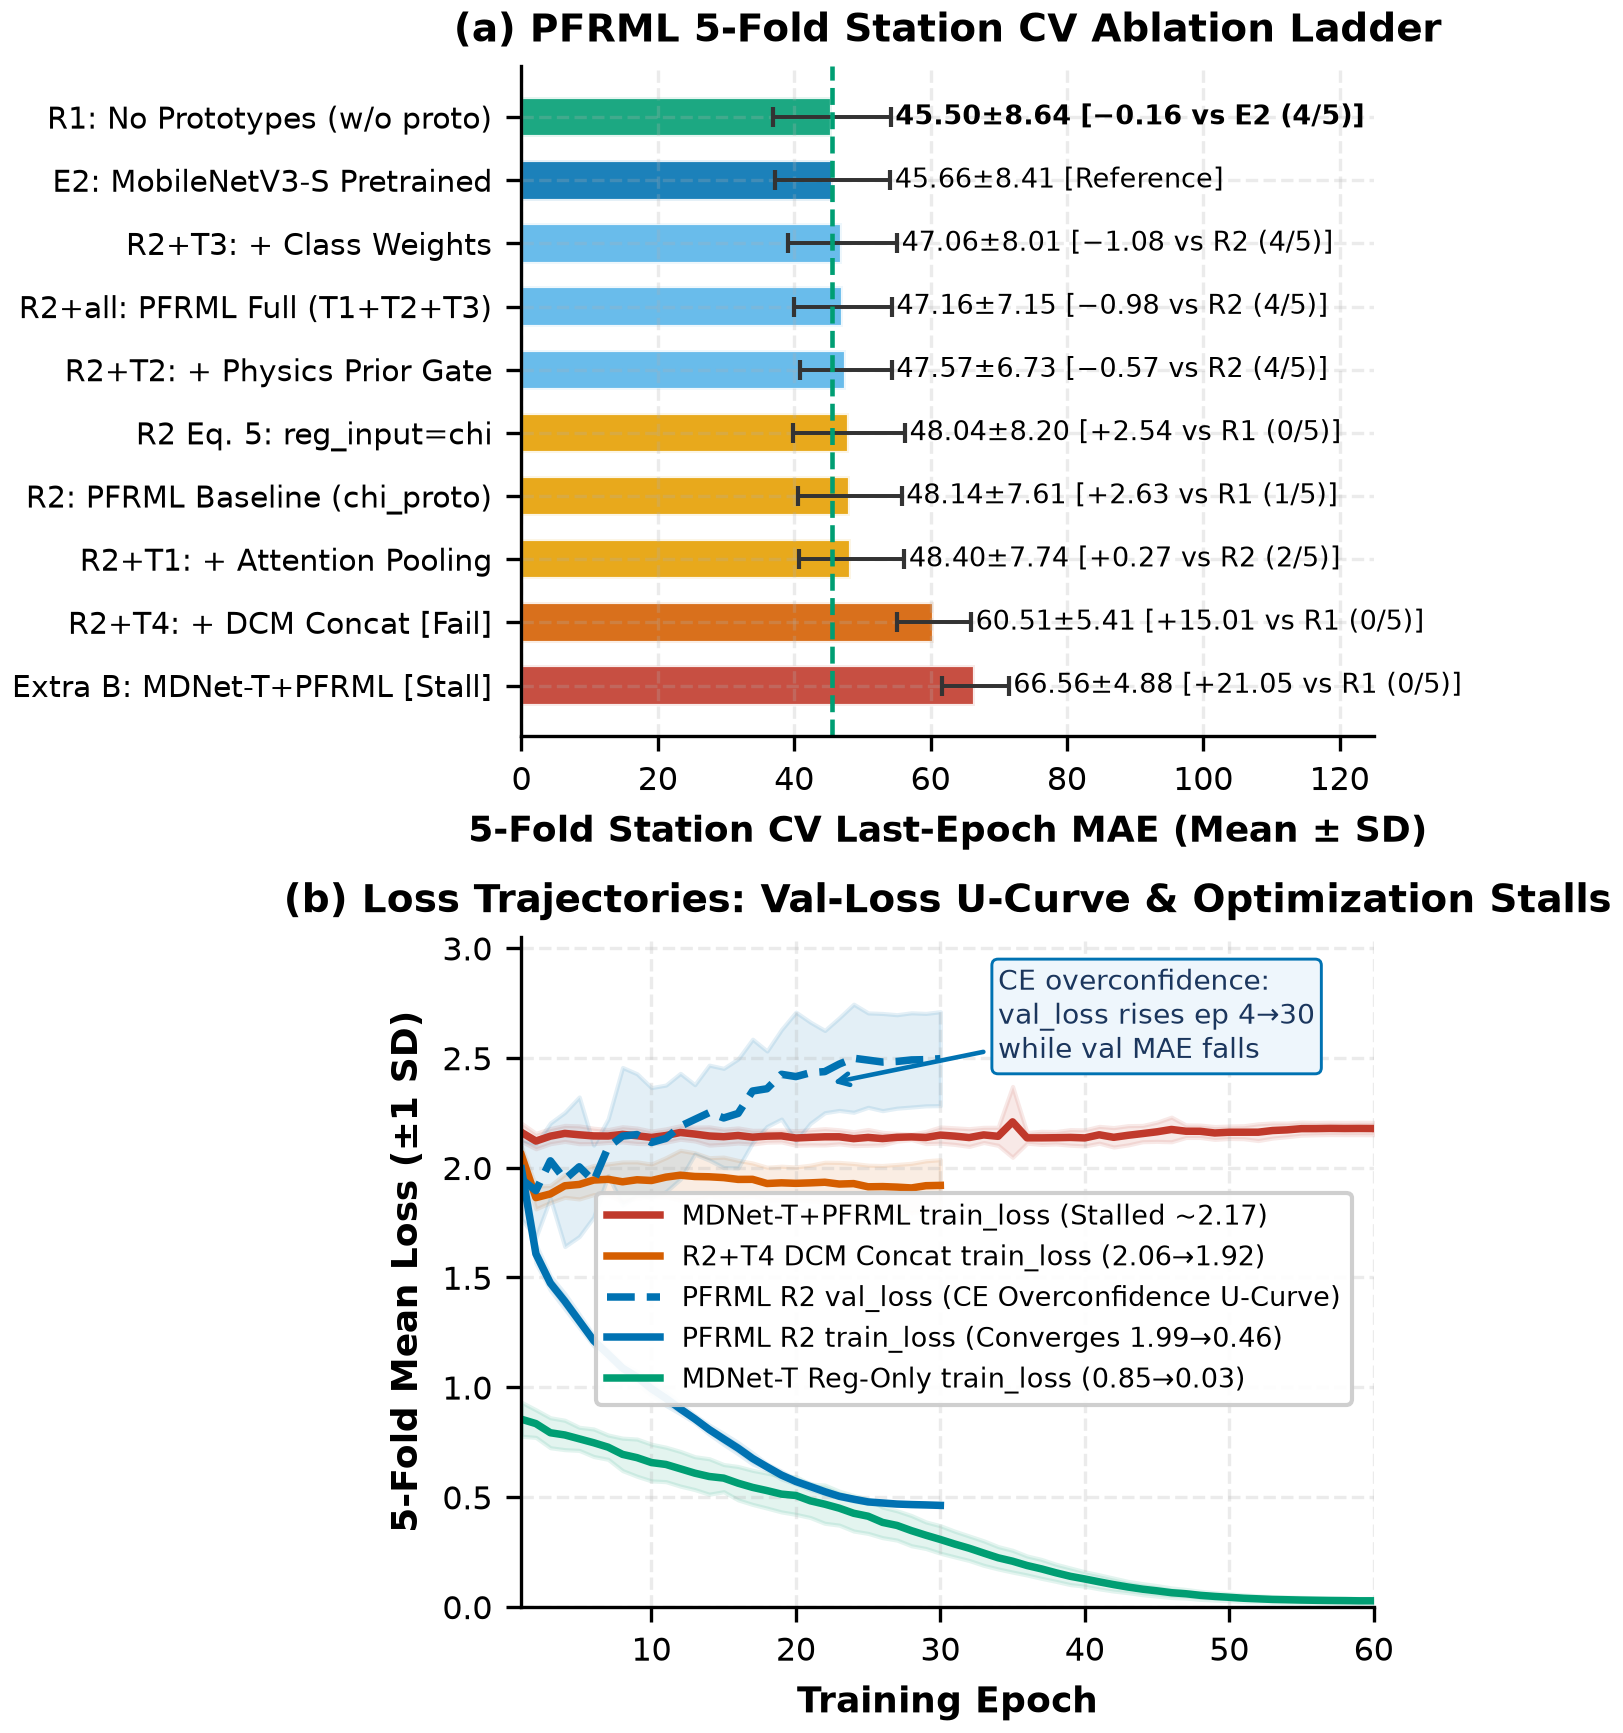
\includegraphics[width=\columnwidth]{figures/ieee_fig4_pfrml_collapse.png}
  \caption{
    PFRML 5-fold ablation ladder and per-epoch loss/MAE trajectories
    illustrating the cross-entropy validation-loss U-curve and optimization
    stalls.
  }
  \label{fig:pfrml_collapse}
\end{figure}

\subsection{
  Multimodal Fusion Under 25 km Spatial-Cluster CV and CMA-3 Early Stopping (E5)
}
\label{subsec:results_fusion_cv}

\begin{table*}[t]
  \centering
  \caption{
    Multimodal Fusion Under 5-Fold 25~km Spatial-Cluster Cross-Validation
    ($n = 8,176$, Authoritative Last-Epoch Metrics) Evaluated Normally and With
    Metadata Zeroed (meta-off). Skill Is Relative to the Constant Median
    Baseline (Spatial-Cluster MAE $= 66.14$).
  }
  \label{tab:fusion_cv}
  \footnotesize
  \setlength{\tabcolsep}{3.8pt}
  \resizebox{\textwidth}{!}{%
    \begin{tabular}{llccccccccccc}
      \toprule
      \textbf{Model / Fusion Variant}                               & \textbf{Eval Mode} &   \textbf{Last-Ep MAE}    &   \textbf{Skill}   &       \textbf{Diff vs.\ E1 (Won)}        &       \textbf{Diff vs.\ E2 (Won)}        &      \textbf{F0 / F1 / F2 / F3 / F4 MAE}       &  \textbf{RMSE}   &   \textbf{PLCC}   &   \textbf{SRCC}   & $\boldsymbol{R^2}$ &   \textbf{Acc}    & $\boldsymbol{\pm 1}$\textbf{Acc} \\
      \midrule
      Constant Median (\texttt{E0\_median})                         & Baseline           &     $66.14 \pm 5.60$      &     $+0.0000$      &         $+20.14 \pm 1.00$ (0/5)          &         $+15.46 \pm 1.04$ (0/5)          &     72.22 / 59.91 / 64.20 / 71.86 / 62.53      &     $88.00$      &     $0.0000$      &     $0.0000$      &     $-0.0168$      &     $0.2154$      &             $0.6500$             \\
      Metadata MLP (\texttt{E1\_metadata\_mlp})                     & Meta Only          &     $46.00 \pm 7.33$      &     $+0.3045$      &          $+0.00 \pm 0.00$ (---)          &          $-4.68 \pm 1.22$ (5/5)          &     55.86 / 37.61 / 43.39 / 51.05 / 42.10      &     $70.09$      &     $0.6257$      &     $0.7147$      &      $0.3647$      &     $0.4183$      &             $0.8603$             \\
      MobileNetV3-S (\texttt{E2\_spatial})                          & Image Only         &     $50.69 \pm 5.60$      &     $+0.2337$      &          $+4.68 \pm 1.22$ (0/5)          &          $+0.00 \pm 0.00$ (---)          &     57.38 / 42.62 / 51.64 / 53.57 / 48.21      &     $77.65$      &     $0.5301$      &     $0.6328$      &      $0.2142$      &     $0.3739$      &             $0.8082$             \\
      \midrule
      Fusion PFRML Full ($p_{\text{drop}} = 0.3$, 30ep)             & Normal             &     $51.68 \pm 6.31$      &     $+0.2187$      &          $+5.68 \pm 1.11$ (0/5)          &          $+1.00 \pm 0.82$ (2/5)          &     61.20 / 44.39 / 52.01 / 52.89 / 47.91      &     $78.71$      &     $0.5377$      &     $0.6608$      &      $0.1883$      &     $0.3387$      &             $0.7727$             \\
      \quad -- Metadata Zeroed                                      & \texttt{meta\_off} &     $54.94 \pm 5.80$      &     $+0.1694$      &          $+8.94 \pm 1.24$ (0/5)          &          $+4.25 \pm 0.76$ (0/5)          &     63.66 / 48.35 / 55.48 / 55.96 / 51.25      &     $82.15$      &     $0.4883$      &     $0.5901$      &      $0.1121$      &     $0.3387$      &             $0.7727$             \\
      Fusion R1 Neck ($p_{\text{drop}} = 0.3$, 30ep)                & Normal             &     $49.18 \pm 6.63$      &     $+0.2565$      &          $+3.18 \pm 1.12$ (1/5)          &          $-1.51 \pm 0.72$ (4/5)          &     58.44 / 40.93 / 50.40 / 51.04 / 45.07      &     $75.83$      &     $0.5741$      &     $0.6722$      &      $0.2484$      &     $0.3769$      &             $0.8245$             \\
      \quad -- Metadata Zeroed                                      & \texttt{meta\_off} &     $52.28 \pm 5.95$      &     $+0.2096$      &          $+6.28 \pm 1.23$ (0/5)          &          $+1.60 \pm 0.56$ (0/5)          &     60.55 / 44.90 / 53.56 / 53.93 / 48.48      &     $78.89$      &     $0.5266$      &     $0.6112$      &      $0.1839$      &     $0.3483$      &             $0.7951$             \\
      Fusion R1 Neck ($p_{\text{drop}} = 0.0$, 30ep)                & Normal             &     $47.45 \pm 6.71$      &     $+0.2827$      &          $+1.44 \pm 1.28$ (1/5)          &          $-3.24 \pm 0.79$ (5/5)          &     56.85 / 38.97 / 49.12 / 48.74 / 43.55      &     $73.88$      &     $0.5993$      &     $0.6994$      &      $0.2869$      &     $0.3956$      &             $0.8358$             \\
      \quad -- Metadata Zeroed                                      & \texttt{meta\_off} &     $53.54 \pm 5.49$      &     $+0.1906$      &          $+7.54 \pm 1.58$ (0/5)          &          $+2.85 \pm 1.04$ (0/5)          &     61.17 / 45.78 / 52.35 / 54.07 / 54.31      &     $79.81$      &     $0.5247$      &     $0.6041$      &      $0.1624$      &     $0.3335$      &             $0.7860$             \\
      \midrule
      \textbf{Fusion R1 Neck ($p_{\text{drop}} = 0.0$, CMA-3 ep 7)} & \textbf{Normal}    & $\mathbf{44.40 \pm 7.30}$ & $\mathbf{+0.3288}$ & $\mathbf{-1.60 \pm 0.59}$ (\textbf{5/5}) & $\mathbf{-6.29 \pm 1.07}$ (\textbf{5/5}) & \textbf{55.09 / 35.76 / 43.09 / 47.36 / 40.69} & $\mathbf{69.68}$ & $\mathbf{0.6395}$ & $\mathbf{0.7330}$ & $\mathbf{0.3674}$  & $\mathbf{0.4318}$ &        $\mathbf{0.8640}$         \\
      \quad -- Metadata Zeroed                                      & \texttt{meta\_off} &     $52.58 \pm 5.06$      &     $+0.2051$      &          $+6.58 \pm 1.49$ (0/5)          &          $+1.90 \pm 1.05$ (1/5)          &     58.20 / 45.16 / 50.39 / 55.80 / 53.35      &     $78.16$      &     $0.5470$      &     $0.6240$      &      $0.1988$      &     $0.3404$      &             $0.7936$             \\
      \bottomrule
    \end{tabular}%
  }
\end{table*}

Table~\ref{tab:fusion_cv} evaluates multimodal fusion under the stricter 25~km
spatial-cluster CV protocol:
\begin{enumerate}
  \item \textbf{Prototype-free R1 fusion outperforms full PFRML fusion:}
        Consistent with our vision-only ladder, fusing the prototype-free R1
        neck ($p_{\text{drop}} = 0.3$, $49.18 \pm 6.63$ MAE) beats fusing the
        full PFRML prototype neck ($p_{\text{drop}} = 0.3$, $51.68 \pm 6.31$
        MAE) by 2.50 MAE points at 30 epochs.
  \item \textbf{30-epoch fusion overfits training cluster coordinates after
        epoch~7:} Training R1 fusion without modality dropout for 30 epochs
        ($p_{\text{drop}} = 0.0$) reaches $47.45 \pm 6.71$ MAE at epoch~30
        (beating image-only MobileNetV3-Small at $50.69 \pm 5.60$ on 5/5 folds,
        but trailing Metadata MLP at $46.00 \pm 7.33$). Inspection of its 5-fold
        validation trajectory reveals that validation MAE drops rapidly from
        57.17 (epoch~1) to a minimum of \textbf{45.74 $\pm$ 6.78 at epoch
        $N = 7$} ($\text{CMA-3} = 46.26$) before drifting upward to 48.11
        (epoch~20) and 47.45 (epoch~30) as the joint MLP overfits training
        cluster coordinates.
  \item \textbf{Early-stopped 7-epoch fusion wins all 5/5 folds against both
        single modalities:} Retraining a fresh 7-epoch cosine schedule
        (\texttt{E5\_fusion\_r1\_p00\_ep7}) achieves \textbf{44.40 $\pm$ 7.30
        MAE} ($\text{Skill} = +0.3288$, $R^2 = 0.3674$, $\text{SRCC} = 0.7330$,
        $\text{Acc} = 0.4318$), beating Metadata MLP by \textbf{$-$1.60 $\pm$
        0.59 MAE (5/5 folds won)} and image-only MobileNetV3-Small by
        \textbf{$-$6.29 $\pm$ 1.07 MAE (5/5 folds won)}. However, zeroing
        metadata at evaluation time degrades MAE to $52.58 \pm 5.06$ (vs.\ 50.69
        for standalone image-only), demonstrating that even with the detached
        auxiliary vision head ($\text{SRCC} = 0.6240$), the shared regression
        MLP still places heavy weight on the metadata embedding.
\end{enumerate}

\subsection{
  One-Shot Held-Out Test and Unseen-Region ($> 25\text{ km}$) Generalization
}
\label{subsec:results_final_test}

\begin{table*}[t]
  \centering
  \caption{
    One-Shot Final Evaluation on the Held-Out Full Test Set ($n = 2,920$, 729
    Stations) and Unseen-Region Subset ($> 25$~km From Any Training Station,
    $n = 717$, 205 Stations). All Neural Models Trained Once on All 8,176
    Training Images (Seed 42) and Evaluated at the Last Epoch. 95\% CIs Use
    1,000-Resample Station-Level Cluster Bootstrap.
  }
  \label{tab:final_test}
  \footnotesize
  \setlength{\tabcolsep}{4.2pt}
  \resizebox{\textwidth}{!}{%
    \begin{tabular}{llcccccccccccc}
      \toprule
      \textbf{Final Model (ID)}                  & \textbf{Architecture (Schedule)} & \textbf{Eval Split} & $\boldsymbol{n}$ (\textbf{St.}) &  \textbf{MAE [95\% Station CI]}  &  \textbf{RMSE}   &   \textbf{PLCC}   &   \textbf{SRCC}   & $\boldsymbol{R^2}$ &   \textbf{Acc}    & $\boldsymbol{\pm 1}$\textbf{Acc} & \textbf{MacroF1}  & \textbf{TailMAE} &  \textbf{TailF1}  \\
      \midrule
      Final Fusion R1 (\texttt{F\_FUSION\_R1})   & R1 Neck + Meta MLP (7ep)         &      Full Test      &           2920 (729)            & $\mathbf{35.77}\;[30.47, 42.72]$ & $\mathbf{51.07}$ & $\mathbf{0.7943}$ & $\mathbf{0.7941}$ & $\mathbf{0.6070}$  & $\mathbf{0.4565}$ &        $\mathbf{0.8938}$         & $\mathbf{0.4150}$ &     $76.92$      & $\mathbf{0.2899}$ \\
      Metadata MLP (\texttt{E1\_metadata\_mlp})  & GPS + Month MLP (40ep)           &      Full Test      &           2920 (729)            &     $40.34\;[34.45, 48.31]$      &     $57.70$      &     $0.7098$      &     $0.7344$      &      $0.4982$      &     $0.4096$      &             $0.8873$             &     $0.3397$      & $\mathbf{76.82}$ &     $0.1362$      \\
      Final Image-Only (\texttt{F\_E2})          & MobileNetV3-S (30ep)             &      Full Test      &           2920 (729)            &     $41.12\;[33.97, 50.79]$      &     $61.95$      &     $0.6749$      &     $0.7071$      &      $0.4215$      &     $0.4240$      &             $0.8620$             &     $0.3723$      &     $96.41$      &     $0.2252$      \\
      Final PFRML Full (\texttt{F\_PFRML\_full}) & PFRML T1+T2+T3 (30ep)            &      Full Test      &           2920 (729)            &     $45.04\;[37.51, 54.04]$      &     $68.56$      &     $0.6039$      &     $0.6574$      &      $0.2914$      &     $0.3986$      &             $0.8134$             &     $0.3687$      &     $96.54$      &     $0.2752$      \\
      Final Fusion Meta-Off (\texttt{meta\_off}) & R1 Fusion ($m_i = 0$, 7ep)       &      Full Test      &           2920 (729)            &     $47.56\;[39.57, 58.12]$      &     $66.12$      &     $0.6936$      &     $0.6757$      &      $0.3411$      &     $0.3428$      &             $0.7897$             &     $0.2556$      &     $119.80$     &     $0.0805$      \\
      \midrule
      Final Fusion R1 (\texttt{F\_FUSION\_R1})   & R1 Neck + Meta MLP (7ep)         &      $> 25$~km      &            717 (205)            & $\mathbf{39.22}\;[30.85, 47.74]$ & $\mathbf{50.68}$ & $\mathbf{0.6464}$ & $\mathbf{0.6696}$ & $\mathbf{0.3743}$  &     $0.3473$      &             $0.7741$             &     $0.2352$      & $\mathbf{86.00}$ &     $0.0000$      \\
      Final Image-Only (\texttt{F\_E2})          & MobileNetV3-S (30ep)             &      $> 25$~km      &            717 (205)            &     $39.60\;[28.06, 54.03]$      &     $54.56$      &     $0.5689$      &     $0.5623$      &      $0.2747$      & $\mathbf{0.4003}$ &        $\mathbf{0.8368}$         & $\mathbf{0.2743}$ &     $116.42$     &     $0.0000$      \\
      Final Fusion Meta-Off (\texttt{meta\_off}) & R1 Fusion ($m_i = 0$, 7ep)       &      $> 25$~km      &            717 (205)            &     $44.88\;[32.15, 58.48]$      &     $59.60$      &     $0.5091$      &     $0.5460$      &      $0.1346$      &     $0.3333$      &             $0.7699$             &     $0.2165$      &     $121.83$     &     $0.0000$      \\
      Final PFRML Full (\texttt{F\_PFRML\_full}) & PFRML T1+T2+T3 (30ep)            &      $> 25$~km      &            717 (205)            &     $46.79\;[34.22, 61.06]$      &     $66.14$      &     $0.4121$      &     $0.5082$      &     $-0.0660$      &     $0.3291$      &             $0.7448$             &     $0.2221$      &     $123.82$     &     $0.0000$      \\
      Metadata MLP (\texttt{E1\_metadata\_mlp})  & GPS + Month MLP (40ep)           &      $> 25$~km      &            717 (205)            &     $49.84\;[40.18, 58.81]$      &     $65.31$      &     $0.3797$      &     $0.4954$      &     $-0.0393$      &     $0.2929$      &             $0.7476$             &     $0.2004$      &     $88.83$      &     $0.0000$      \\
      \bottomrule
    \end{tabular}%
  }
\end{table*}

\begin{table}[t]
  \centering
  \caption{
    Paired Station-Level Cluster Bootstrap MAE Differences (Model A Minus Model
    B and 95\% CIs, 1,000 Resamples, Seed 42) on Full Test ($n = 2,920$) and
    Unseen-Region Subset ($> 25$~km, $n = 717$).
  }
  \label{tab:paired_bootstrap}
  \footnotesize
  \setlength{\tabcolsep}{3.2pt}
  \resizebox{\columnwidth}{!}{%
    \begin{tabular}{llcc}
      \toprule
      \textbf{Model A vs.\ Model B}                                 & \textbf{Split}   &          \textbf{MAE Diff}           &       \textbf{95\% Station CI}        \\
      \midrule
      \texttt{F\_E2} vs.\ \texttt{F\_PFRML\_full}                   & Full / $> 25$~km & $\mathbf{-3.92}$ / $\mathbf{-7.18}$  & $[-6.27, -1.58]$ / $[-11.92, -2.53]$  \\
      \texttt{F\_E2} vs.\ \texttt{F\_FUSION\_R1}                    & Full / $> 25$~km &          $+5.35$ / $+0.38$           &  $[+2.26, +8.62]$ / $[-5.99, +8.09]$  \\
      \texttt{F\_E2} vs.\ \texttt{F\_FUSION\_meta\_off}             & Full / $> 25$~km &      $\mathbf{-6.44}$ / $-5.28$      & $[-9.39, -3.22]$ / $[-10.67, +0.00]$  \\
      \texttt{F\_E2} vs.\ \texttt{E1\_metadata\_mlp}                & Full / $> 25$~km &          $+0.77$ / $-10.24$          & $[-3.46, +4.78]$ / $[-20.50, +0.86]$  \\
      \texttt{F\_PFRML\_full} vs.\ \texttt{F\_FUSION\_R1}           & Full / $> 25$~km &          $+9.26$ / $+7.57$           & $[+6.06, +12.52]$ / $[+1.46, +14.29]$ \\
      \texttt{F\_PFRML\_full} vs.\ \texttt{F\_FUSION\_meta\_off}    & Full / $> 25$~km &          $-2.52$ / $+1.90$           &  $[-6.13, +1.27]$ / $[-2.35, +6.01]$  \\
      \texttt{F\_PFRML\_full} vs.\ \texttt{E1\_metadata\_mlp}       & Full / $> 25$~km &          $+4.69$ / $-3.06$           & $[+0.24, +9.10]$ / $[-14.90, +8.29]$  \\
      \texttt{F\_FUSION\_R1} vs.\ \texttt{F\_FUSION\_meta\_off}     & Full / $> 25$~km &     $\mathbf{-11.79}$ / $-5.66$      & $[-16.00, -7.74]$ / $[-11.75, +0.92]$ \\
      \texttt{F\_FUSION\_R1} vs.\ \texttt{E1\_metadata\_mlp}        & Full / $> 25$~km & $\mathbf{-4.57}$ / $\mathbf{-10.63}$ & $[-8.31, -1.26]$ / $[-18.78, -2.59]$  \\
      \texttt{F\_FUSION\_meta\_off} vs.\ \texttt{E1\_metadata\_mlp} & Full / $> 25$~km &          $+7.21$ / $-4.96$           & $[+1.56, +12.49]$ / $[-16.73, +5.42]$ \\
      \bottomrule
    \end{tabular}%
  }
\end{table}

Tables~\ref{tab:final_test} and~\ref{tab:paired_bootstrap} report the one-shot
held-out test evaluation and paired station-bootstrap CIs (see
Fig.~\ref{fig:fusion_test}):
\begin{enumerate}
  \item \textbf{Final Fusion R1 (\texttt{F\_FUSION\_R1}) significantly beats
        every single-modality model on the full test set:} With a test MAE of
        \textbf{35.77~[30.47, 42.72]} ($\text{RMSE} = 51.07$,
        $\text{PLCC} = 0.7943$, $\text{SRCC} = 0.7941$, $R^2 = 0.6070$,
        $\text{Acc} = 0.4565$, $\pm 1\text{Acc} = 0.8938$,
        $\text{MacroF1} = 0.4150$), Final Fusion R1 outperforms Metadata MLP by
        \textbf{$-$4.57~[$-$8.31, $-$1.26] MAE}, image-only MobileNetV3-Small
        (\texttt{F\_E2}) by \textbf{$-$5.35~[$-$8.62, $-$2.26] MAE}, and Final
        PFRML Full (\texttt{F\_PFRML\_full}) by \textbf{$-$9.26~[$-$12.52,
        $-$6.06] MAE} (all 95\% CIs strictly excluding zero).
  \item \textbf{Plain pretrained MobileNetV3-Small (\texttt{F\_E2})
        significantly beats Final PFRML Full on both test partitions:}
        Confirming our 5-fold CV finding, \texttt{F\_E2} outperforms
        \texttt{F\_PFRML\_full} by \textbf{$-$3.92~[$-$6.27, $-$1.58] MAE} on
        the full test set (41.12 vs.\ 45.04) and by \textbf{$-$7.18~[$-$11.92,
        $-$2.53] MAE} on \texttt{test\_gt25km} (39.60 vs.\ 46.79, where
        \texttt{F\_PFRML\_full} falls to $R^2 = -0.0660$).
  \item \textbf{Far from training stations ($> 25$~km), visual and fused models
        remain stable while metadata collapses:} On \texttt{test\_gt25km}
        ($n = 717$, 205 stations), \texttt{F\_FUSION\_R1} achieves the lowest
        MAE (\textbf{39.22~[30.85, 47.74]}, $R^2 = 0.3743$,
        $\text{SRCC} = 0.6696$), significantly beating Metadata MLP ($49.84$,
        $R^2 = -0.0393$) by \textbf{$-$10.63~[$-$18.78, $-$2.59] MAE} and
        \texttt{F\_PFRML\_full} by \textbf{$-$7.57~[$-$14.29, $-$1.46] MAE},
        while statistically tying standalone vision \texttt{F\_E2} ($39.60$,
        $R^2 = 0.2747$, paired difference $+0.38\;[-5.99, +8.09]$). Standalone
        vision \texttt{F\_E2} actually achieves slightly lower MAE at $> 25$~km
        (39.60) than on the full test set (41.12), with a $-10.24$-point MAE
        advantage over Metadata MLP whose 95\% CI slightly crosses zero
        ($[-20.50, +0.86]$).
  \item \textbf{Zeroing metadata at test time reveals continued location
        dependence:} When metadata is zeroed out at evaluation time
        (\texttt{F\_FUSION\_R1\_meta\_off}), full-test MAE jumps by
        $+11.79\;[+7.74, +16.00]$ points from 35.77 to 47.56 (44.88 on
        \texttt{test\_gt25km}), which is significantly worse than standalone
        \texttt{F\_E2} (41.12, paired difference $-6.44\;[-9.39, -3.22]$ on full
        test; $-5.28\;[-10.67, +0.00]$ on \texttt{test\_gt25km}). Thus,
        multimodal fusion effectively combines visual and geospatial signals
        when both are present, but does not eliminate reliance on the metadata
        branch.
\end{enumerate}

\begin{figure}[t]
  \centering
  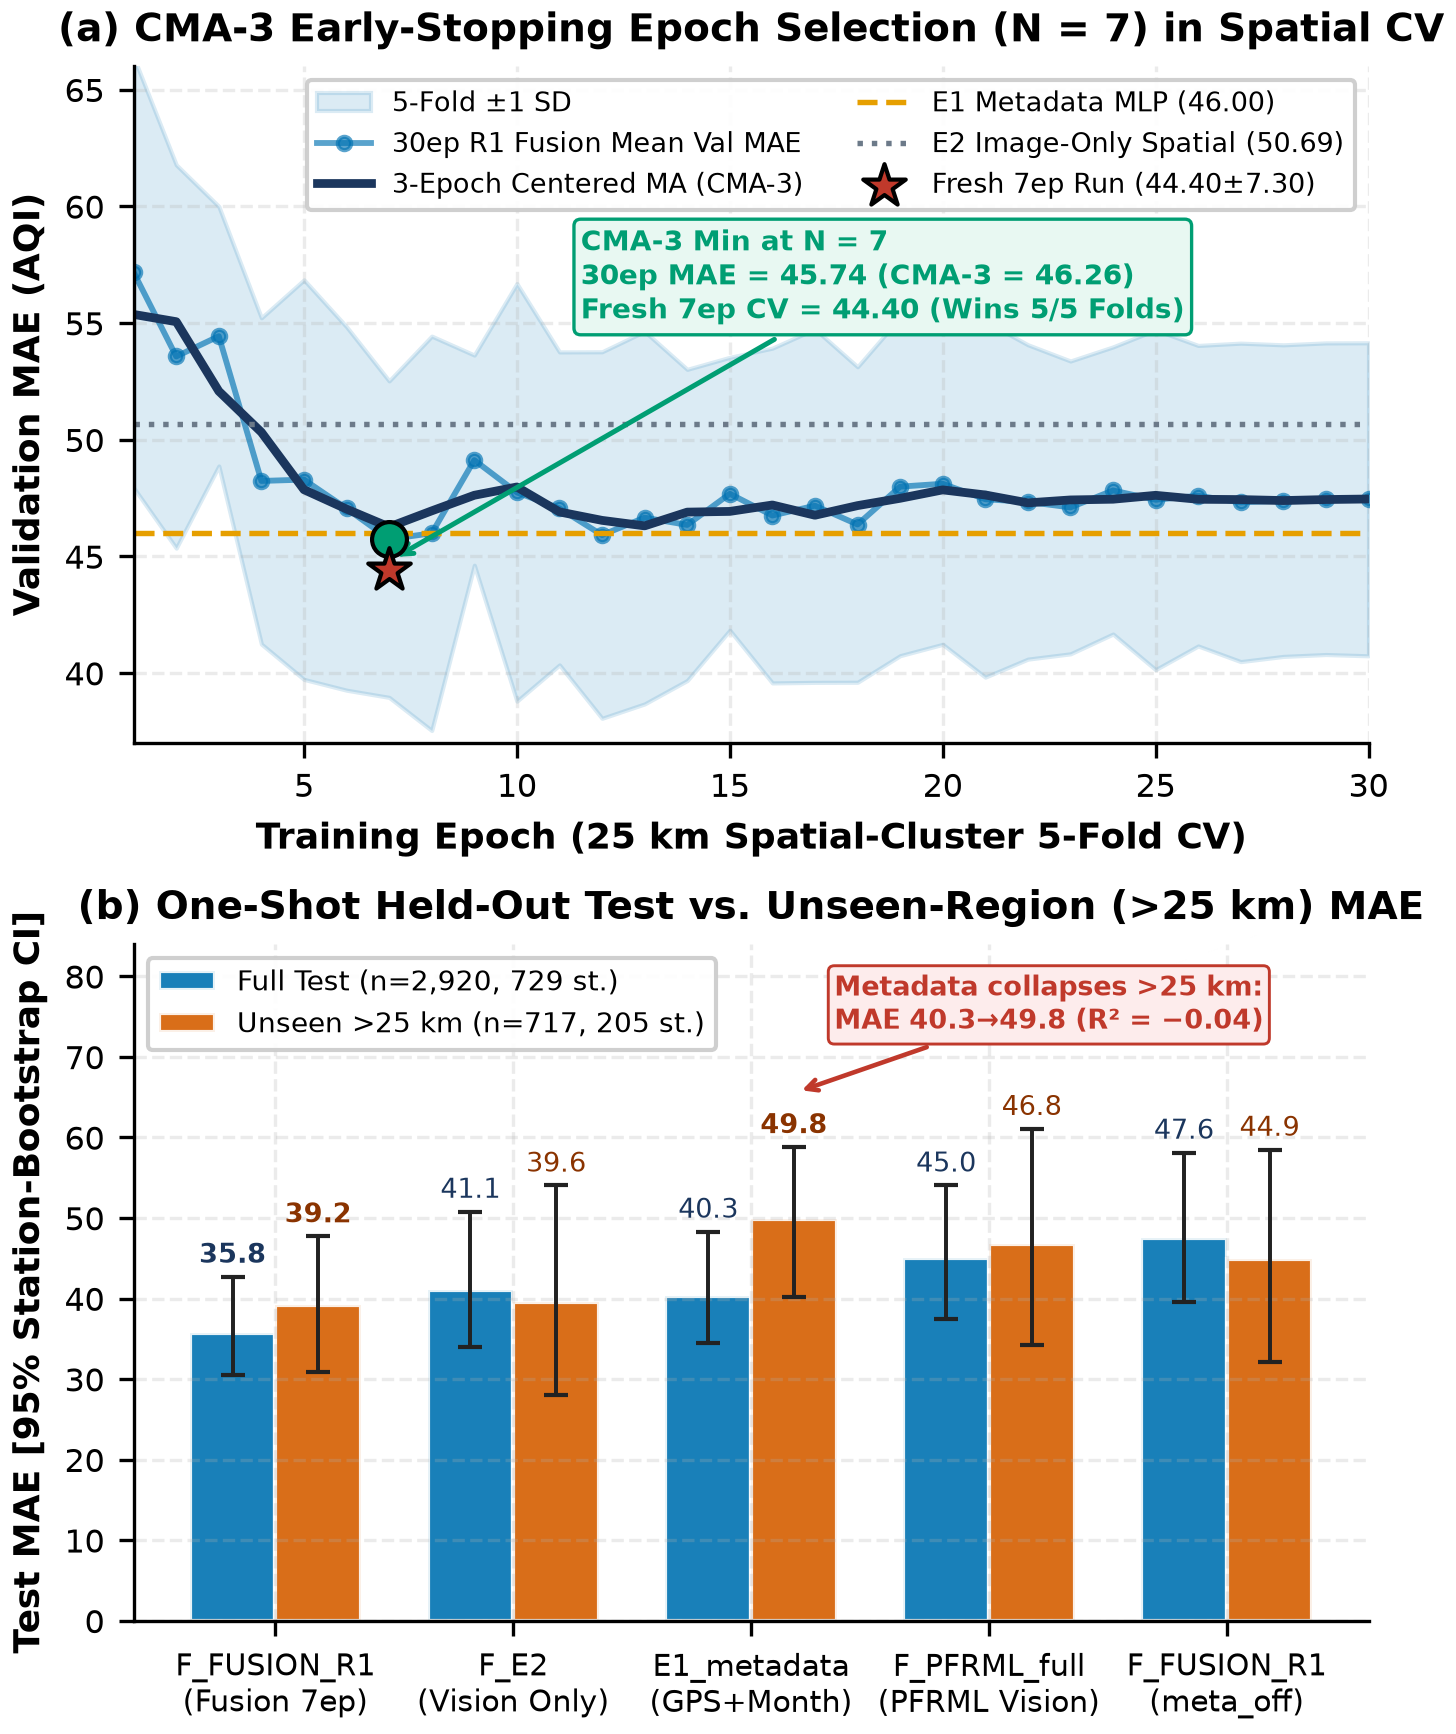
\includegraphics[width=\columnwidth]{figures/ieee_fig5_fusion_test.png}
  \caption{
    Early-stopping epoch selection (CMA-3 at $N = 7$) in 25~km spatial-cluster
    CV and final one-shot test vs.\ $> 25$~km generalization with 95\%
    station-bootstrap CIs.
  }
  \label{fig:fusion_test}
\end{figure}

\subsection{Discussion, Limitations, and Threats to Validity}
\label{subsec:discussion_limitations}

To maintain scientific rigor, we explicitly distinguish between
\textbf{established empirical findings} (supported by 5-fold consistency or
paired 95\% station-bootstrap confidence intervals excluding zero) and
\textbf{hypotheses} (plausible mechanistic explanations that were not isolated
by separate experiments):
\begin{itemize}
  \item \textbf{Established vs.\ Hypothesis on Prototype Multitask
        Regularization:} It is an \textit{established finding} on our global
        PM25Vision setup with a MobileNetV3-Small backbone that removing PFRML's
        prototype classification branch (R1, 45.50 CV MAE) beats both the
        prototype-weighted head (R2, 48.14) and the literal Eq.~5 head (48.04),
        and that plain pretrained MobileNetV3-Small (\texttt{F\_E2}, 41.12 test
        MAE) significantly beats \texttt{F\_PFRML\_full} (45.04, CI
        $[-6.27, -1.58]$). Notice that this does \textit{not} imply PFRML fails
        in general; rather, our \textit{hypothesis} for why prototypes cost
        accuracy here is that 6-class AQI separability across diverse global
        street cameras plateaus near $\sim 41\%$ accuracy, causing the
        cross-entropy loss to compete with regression for shared representation
        capacity, become overconfident after epoch~6, and inject noisy 6-class
        probability weights into the regression head.
  \item \textbf{Established vs.\ Hypothesis on Multimodal Shortcut Reliance:} It
        is an \textit{established finding} that early-stopped
        \texttt{F\_FUSION\_R1} (35.77 test MAE) significantly outperforms both
        single modalities on the full test set and beats metadata-only beyond
        25~km ($-10.63\;[-18.78, -2.59]$), yet degrades to 47.56 MAE when
        metadata is zeroed (\texttt{meta\_off}). Our \textit{hypothesis} is that
        the low-dimensional Metadata MLP branch memorizes regional pollution
        levels much faster than the convolutional/Transformer spine extracts
        subtle Mie scattering gradients, causing the shared regression MLP
        ($256 \to 256 \to 1$) to assign large weights to the metadata embedding
        and suffer a baseline offset shift when metadata is zeroed.
  \item \textbf{Unresolved Tension Between Spatial-Cluster CV and the
        $> 25$~km Test Subset:} In 5-fold 25~km spatial-cluster CV,
        metadata-only beat image-only on all 5/5 folds ($46.00 \pm 7.33$
        vs.\ $50.69 \pm 5.60$ MAE), whereas on the held-out
        \texttt{test\_gt25km} subset ($n = 717$, 205 stations), image-only
        \texttt{F\_E2} achieved a 10.24-point lower MAE than Metadata MLP (39.60
        vs.\ 49.84, paired 95\% CI $[-20.50, +0.86]$ slightly crossing zero). A
        plausible \textit{hypothesis} is that the 205 remote test stations in
        \texttt{test\_gt25km} have a different geographic distribution and lower
        extreme-tail variance than the training folds (as evidenced by the
        Constant Median Predictor achieving 56.60 MAE on \texttt{test\_gt25km}
        vs.\ 66.14 in spatial-cluster CV).
\end{itemize}

Finally, we highlight six methodological and statistical limitations of this
study:
\begin{enumerate}
  \item \textbf{Single random seed ($\text{seed} = 42$) and 5-fold Wilcoxon
        ceiling:} Because all experiments ran with a single seed across $n = 5$
        folds, run-to-run stochastic optimization variance ($\sim 1\text{--}2$
        MAE points) is not averaged out, and paired Wilcoxon tests cannot reach
        $p < 0.05$ ($p_{\min} = 0.0625$).
  \item \textbf{Same-fold hyperparameter and epoch-selection optimism:} Stage~2
        learning-rate/epoch screening for image baselines used Fold~0 (which is
        included in the 5-fold CV average), and the early-stopping epoch count
        $N = 7$ for 7-epoch R1 fusion ($44.40 \pm 7.30$ CV MAE) was chosen from
        the 5-fold validation curves of 30-epoch R1 fusion. Thus, their CV means
        carry mild selection optimism, and the one-shot held-out test set serves
        as the uncheated verification.
  \item \textbf{Small \texttt{test\_gt25km} sample size ($n = 717$, 205
        stations) and empty extreme-tail $F_1$:} On \texttt{test\_gt25km},
        station-bootstrap CIs span 17--26 MAE points, and every evaluated model
        records $\text{TailF1} = 0.0000$, so tail classification metrics on the
        $> 25$~km subset should not be over-interpreted.
  \item \textbf{Backbone substitutions relative to original papers:} To fit
        laptop GPU memory and $\sim 8.2\text{k}$ training images, our PFRML
        ladder substituted MobileNetV3-Small ($D = 224$, 2-layer Transformer,
        batch size 32, $\text{lr} = 10^{-3}$) for Wang et
        al.'s~\cite{wangPrototypeFeatureRepresentationGuided2026}
        115.2M-parameter ResNet-50 + 12-layer ViT
        ($\text{lr} = 2 \times 10^{-4}$, batch size 16).
  \item \textbf{Apple Silicon \texttt{mps} floating-point non-determinism:}
        While offline evaluation of saved predictions and checkpoints is
        bit-exact, retraining neural models from scratch on the Apple Metal
        Performance Shaders (\texttt{mps}) backend exhibits minor floating-point
        atomic accumulation variance.
  \item \textbf{Scope exclusions and future work:} Due to project time
        constraints, on-device iPhone Core~ML latency benchmarking, Grad-CAM /
        Transformer spatial attention map visualizations, prototype-mixture
        uncertainty calibration plots, decoupled modality learning rates
        ($\text{lr}_{\text{meta}} < \text{lr}_{\text{image}}$), and
        distance-aware post-hoc ensembling of \texttt{F\_E2} and Metadata MLP
        were left for future work.
\end{enumerate}

\section{Conclusion}
\label{sec:conclusion}

This study investigated global street-level Air Quality Index estimation on the
cleaned PM25Vision benchmark (8,176 training images across 2,527 stations; 2,920
test images across 729 stations, including 717 images across 205 stations
located $> 25$~km from any training station) by auditing and adapting two IEEE
Transactions architectures---MDNet~\cite{wangLightweightAirQuality2024} and
PFRML~\cite{wangPrototypeFeatureRepresentationGuided2026}---under strict
station-grouped and 25~km spatial-cluster cross-validation, last-epoch
reporting, and 1,000-resample station-level cluster bootstrapping.

Our experiments provide clear answers to all four research questions. First
(\textbf{RQ1}), non-visual GPS and seasonal metadata
(\texttt{E1\_metadata\_mlp}) creates a potent spatial shortcut near training
cities ($\text{MAE} = 40.34$, $R^2 = 0.4982$ on full test) that collapses
completely in unseen regions $> 25$~km away ($\text{MAE} = 49.84$,
$R^2 = -0.0393$), whereas pure vision (\texttt{F\_E2}, pretrained
MobileNetV3-Small) generalizes across distance (41.12 full test; 39.60 at
$> 25$~km, $R^2 = 0.2747$). Second (\textbf{RQ2}), ImageNet pretraining improves
5-fold station CV MAE by 7.61--9.24 points over from-scratch ResNet-18
($53.27 \pm 7.11$) and from-scratch MDNet-T ($53.29 \pm 6.38$), while our
lightweight MobileNetV3-S + MD-Neck adaptation ($44.92 \pm 8.54$, 1.04M
parameters) and plain MobileNetV3-Small ($45.66 \pm 8.41$, 1.52M parameters)
closely match pretrained ResNet-18 ($44.05 \pm 8.70$, 11.18M parameters). Third
(\textbf{RQ3}), across a 5-fold ablation ladder, PFRML's multi-stage DCM +
Transformer neck without prototypes (R1, $45.50 \pm 8.64$) matches the
pretrained backbone, but enabling the 6-class EMA prototype multitask head (R2,
$48.14 \pm 7.61$; literal Eq.~5 variant, $48.04 \pm 8.20$) degrades continuous
regression, and plain \texttt{F\_E2} significantly beats \texttt{F\_PFRML\_full}
on both the full test set ($-3.92\;[-6.27, -1.58]$) and \texttt{test\_gt25km}
($-7.18\;[-11.92, -2.53]$). Fourth (\textbf{RQ4}), fusing the prototype-free R1
visual neck with metadata under CMA-3 early stopping at $N = 7$ epochs
(\texttt{F\_FUSION\_R1}) achieves the best overall performance on the full test
set ($\text{MAE} = 35.77\;[30.47, 42.72]$, $R^2 = 0.6070$, beating metadata-only
by $-4.57\;[-8.31, -1.26]$ and image-only by $-5.35\;[-8.62, -2.26]$) and ties
image-only beyond 25~km (39.22 vs.\ 39.60, beating metadata-only by
$-10.63\;[-18.78, -2.59]$), although zeroing metadata at evaluation time (47.56
MAE) shows that mitigating shortcut reliance in joint regression heads remains
an open challenge for future decoupled-learning-rate and post-hoc ensembling
designs.

\textbf{Reproducibility:} All experiments were executed at git commit
\texttt{fd7bea3} ($\text{seed} = 42$) on an Apple MacBook Pro (Apple M5 Pro,
24~GB unified memory, macOS-27.2.1-arm64) using Python 3.14.6 and PyTorch 2.14.1
(\texttt{mps} backend, \texttt{fp32}). Every table, paired difference, and
1,000-resample station-bootstrap CI in this report can be regenerated
bit-for-bit offline from the tracked \texttt{results/} snapshot via the
repository's analysis scripts (\texttt{build\_report\_numbers.py} and
\texttt{compare\_final\_models.py}).

\bibliographystyle{IEEEtran}
\bibliography{references}

\end{document}
